\documentclass[../mss.tex]{subfiles}
\begin{document}
\part{Экзамен №2}

\chapter{Элементы тензорного исчисления (повторение, будут в качестве доп.вопросов)}
\que{Локальные векторные базисы, метрические матрицы, преобразования координат.}


\que{Определение тензора, диадные базисы, алгебраические операции с тензорами.}


\que{Симметричные, кососимметричные и ортогональные тензоры. Собственные значения и собственные векторы тензора 2-го ранга.}


\que{Векторное произведение, его свойства, символы Леви-Чивиты.}


\que{Ковариантное дифференцирование тензоров.}


\que{Физические компоненты тензоров.}



\chapter{Соотношения на поверхности сильных разрывов}
\que{Классификация поверхностей раздела. Аксиома о классе функций при переходе через поверхность разрыва. Правило дифференцирования объемного интеграла при наличии поверхности разрыва.}

\paragraph{Классификация поверхностей раздела}
\begin{center}
	\begin{tikzpicture}[node distance=4cm]
		
		\node (start) [block] {Разрывы\\ (поверхность разрыва $S(t)$)};
		
		\node (slab) [block, below left of=start] {Слабые\\ $\mathring{\rho}, \mathring{A}_\alpha, \mathring{B}_\alpha$ - непрерывны по $\mathring{S}$, а их производные - терпят разрыв};
		
		\node (siln) [block, below right of=start] {Сильные\\ Хотя бы одна $\mathring{\rho}, \mathring{A}_\alpha, \mathring{B}_\alpha$ - терпят разрыв};
		
		\node (neper) [block, below left of=siln] {Материальные точки не переходят через $S(t)$};
		\node (per) [block, below right of=siln] {Материальные точки  переходят через $S(t)$};
		\node (per1) [block1, below left of=neper] {Контактный разрыв\\(ОС не меняются)};
		\node (per2) [block1, right of=per1] {Поверхность контакта\\(ОС меняются)};
		
		\node (per3) [block1,right of=per2] {Ударная волна\\(ОС не меняются)};
		\node (per4) [block1, right of=per3] {Фазовое превращение\\(ОС меняются)};
		
		\draw [arrow] (start) -- (slab);
		\draw [arrow] (start) -- (siln);
		\draw [arrow] (siln) -- (neper);
		\draw [arrow] (siln) -- (per);
		
		\draw [arrow] (neper) -- (per1);
		\draw [arrow] (neper) -- (per2);
		
		\draw [arrow] (per) -- (per3);
		\draw [arrow] (per) -- (per4);
	\end{tikzpicture}
\end{center}
\begin{definition}
	Поверхность разрыва $S(t)$, при переходе через которую терпят разрыв сами неизвестные функции $\rho, \mathbf{u},\mathbf{v},\mathbf{T},\mathbf{F},$ и др. называют \textit{ поверхностью сильного разрыва}, если ж е эти функции остаются непрерывными, а терпят разрыв только их первые производные по t и координатам ($\mathbf{\nabla}\rho,\mathbf{\nabla}\otimes \mathbf{u}, \mathbf{\nabla}\otimes \mathbf{v}$ и т.д.), то $S(t)$ называют \textit{поверхностью слабого разрыва}.
\end{definition}
\begin{definition}
	Поверхность сильного разрыва $S(t)$, через которую для $\forall t\in [t_1,t_2]$ не переходят материальные точки, называют
	\textit{поверхностью контактного разрыва}, если определяющие соотношения в областях $V_+(t)$ и $V_-(t)$ одинаковы для всех рассматриваемых $t$, в противном ж е случае ее называют \textit{поверхностью контакта}.
\end{definition}
\begin{definition}
	Поверхность сильного разрыва $S(t)$, через которую при
	$\forall t\in [t_1,t_2]$ переходят материальные точки, называют \textit{поверхностью ударной волны}, если определяющие соотношения одинаковы для всех рассматриваемых $t$, в противном случае $S(t)$ называют \textit{поверхностью фазового перехода}.
\end{definition}

\begin{definition}
	Поверхность разрыва $S(t)$, при переходе через которую
	терпят разрывы радиусы-векторы $\mathbf{x}$ материальных точек $M \in S(t)$, называют \textit{некогерентной}, в противном случае поверхность называют \textit{когерентной}.
\end{definition}

\paragraph{Аксиома о классе функций при переходе через поверхность разрыва}
Рассмотрим далее поверхность сильного разрыва $\mathring{S}(t)$, разделяющую область $\mathring{V}$ в $\mathring{\mathcal{K}}$ на две подобласти $\mathring{V}_+$ и $\mathring{V}_-$.

\begin{definition}
	Пусть имеется функция $A(\mathring{\mathbf{x}},t)$, определенная в области $\mathring{V}$. \textit{Скачком} функции \textit{через поверхность разрыва $\mathring{S}$} называют следующую величину:
	\[
	[A]=\left.A_+\right|_{\mathring{S}}-\left.A_-\right|_{\mathring{S}}
	\]
	где
	\[
	\left.A_{\pm}\right|_{\mathring{S}}=\lim_{
		\begin{aligned}
			&\mathring{\mathbf{x}}\to\mathring{\mathbf{x}}_\Sigma\\
			\mathring{\mathbf{x}}\in&\mathring{V}_{\pm},\mathring{\mathbf{x}}_\Sigma\in\mathring{S}
	\end{aligned}}A_{\pm}(\mathring{\mathbf{x}},t).
	\]
\end{definition}

\begin{axiom}\label{ax17}
	Для сплошной среды, содержащей в $\mathring{\mathcal{K}}$ поверхность разрыва $\mathring{S}(t)$, которая разделяет область $\mathring{V}$ на части $\mathring{V}_+$ и $\mathring{V}_-$, функций $\mathring{\rho}, \mathring{A}_\alpha$ и $\mathring{B}_\alpha$ в системе законов сохранения предполагаются гладкими в $\mathring{V}_+$ и $\mathring{V}_-$:
	\[
	\begin{aligned}
		\mathring{A}_\alpha=\begin{cases}
			\begin{aligned}
				&\mathring{A}_{\alpha+},&\mathring{\mathbf{x}}\in\mathring{V}_+,\\
				&\mathring{A}_{\alpha-},&\mathring{\mathbf{x}}\in\mathring{V}_-,
			\end{aligned}
		\end{cases}
		\mathring{B}_\alpha=\begin{cases}
			\begin{aligned}
				&\mathring{B}_{\alpha+},&\mathring{\mathbf{x}}\in\mathring{V}_+,\\
				&\mathring{B}_{\alpha-},&\mathring{\mathbf{x}}\in\mathring{V}_-,
			\end{aligned}
		\end{cases}
	\end{aligned}
	\]
	а на поверхности разрыва $\mathring{S}(t)$ могут иметь конечный скачок, т.е.
	\[
	\begin{aligned}
		&[\mathring{A}_\alpha] < \infty,&	[\mathring{B}_\alpha] < \infty.
	\end{aligned}
	\]
	Функции $C_\alpha$ в системе законов сохранения энергии также предполагаются гладкими в $\mathring{V}_+$ и $\mathring{V}_-$, а на поверхности разрыва могут иметь неограниченный скачок типа скачка $\delta$-функции:
	\[
	\begin{aligned}
		&\mathring{\rho}C_\alpha=\mathring{\rho}\tilde{C}_\alpha+\mathring{C}_{\alpha\Sigma}\delta(\mathring{\mathbf{x}}_\Sigma-\mathring{\mathbf{x}}),&\tilde{C}_\alpha=\begin{cases}
			\begin{aligned}
				&\mathring{C}_{\alpha+},&\mathring{\mathbf{x}}\in\mathring{V}_+,\\
				&\mathring{C}_{\alpha-},&\mathring{\mathbf{x}}\in\mathring{V}_-,
			\end{aligned}
		\end{cases}
	\end{aligned}
	\]
	где $\mathring{C}_{\alpha\Sigma}(\mathring{\mathbf{x}}_\Sigma,t)$ - конечная гладкая по $\mathring{S}(t)$ функция, удовлетворяющая условию:
	\[
	\int_{\mathring{V}}\mathring{C}_{\alpha\Sigma}\delta(\mathring{\mathbf{x}}_\Sigma-\mathring{\mathbf{x}})d\mathring{V}=\int_{\mathring{S}}\mathring{C}_{\alpha\Sigma}d\mathring{\Sigma}
	\]
	Функция $\mathring{C}_{4\Sigma}$ состоит из двух слагаемых: скачка производства энтропии за счет внешних источников $\mathring{\bar{C}}_{4\Sigma}$ и скачка производства энтропии за
	счет внутренних источников $\mathring{C}_{4\Sigma}^*$, который полагают всегда неотрицательным:
	\[
	\mathring{C}_{4\Sigma}=\mathring{\bar{C}}_{4\Sigma}+\mathring{C}_{4\Sigma}^*,~~~\mathring{C}_{4\Sigma}^*\geq 0.
	\]
\end{axiom}
	\paragraph{Правило дифференцирования объемного интеграла при наличии поверхности разрыва}
	\begin{theorem}
		Для любых функций $\mathring{A}_\alpha$, определенных в области $\mathring{V}$ с поверхность разрыва $\mathring{S}$ и удовлетворяющих аксиоме \ref{ax17}, имеет место \textit{правило дифференцирования объемного интеграла}:
		\[
		\frac{\partial}{\partial t}\int_{\mathring{V}}\mathring{\rho}\mathring{A}_\alpha d\mathring{V}=\int_{\mathring{V}}\mathring{\rho}	\frac{\partial\mathring{A}_\alpha}{\partial t}d\mathring{V}-\int_{\mathring{S}}\left(\mathring{\rho}_+\mathring{A}_{\alpha+}-\mathring{\rho}_-\mathring{A}_{\alpha-}\right)\mathring{D}d\mathring{\Sigma},
		\]
		где
		\[
			\mathring{D}=\mathring{\mathbf{c}}\cdot\mathring{\mathbf{n}}
		\]
		- нормальная скорость движения поверхности разрыва.
	\end{theorem}
\que{Соотношения на поверхностях сильных разрывов в материальном описании.}


Пусть поверхность разрыва $S(t)$ является когерентной, рассмотрим ее образ в $\mathring{\mathcal{K}}$ - поверхность разрыва $\mathring{S}$ и точку $\mathcal{M}\in\mathring{S}$. Построим специальную область $\mathring{V}_h$, называемую \textit{окрестностью поверхности разрыва} и содержащую точку $\mathcal{M}$ (Рис. \ref{risun}). 

% TODO: \usepackage{graphicx} required

\begin{figure}[h!]
	\centering
	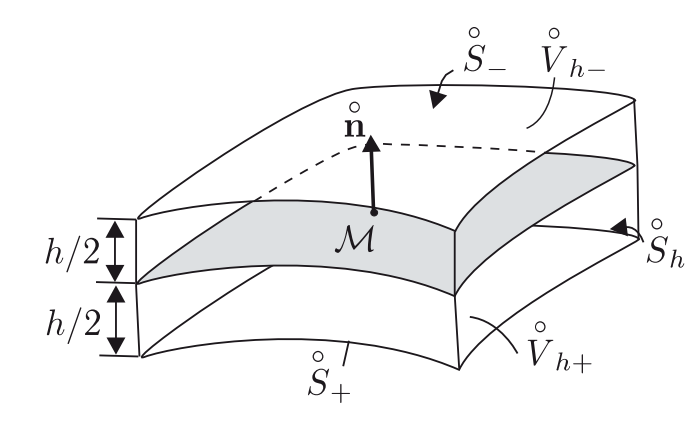
\includegraphics[width=0.7\linewidth]{semester8/img/screenshot001}
	\caption{Область для вывода условий на поверхности разрыва}
	\label{risun}
\end{figure}

Для построения области $\mathring{V}_h$	выберем часть $\mathring{\Sigma}_h$ поверхности $\mathring{S}$, так что $\mathcal{M}\in\mathring{\Sigma}_h$, и введем криволинейные координаты $X^i$ таким образом, что линии $X^1,X^2$ принадлежат поверхности $\mathring{S}$, а линии $X^3$ направлены по нормали к $\mathring{S}$. Область $\mathring{V}_h$ ограничена поверхностью $\partial\mathring{V}_h$, состоящей из боковых поверхностей $\mathring{\Sigma}_{h\pm}$ (их уравнения $X^3=\pm h/2$), торцевых поверхностей $\mathring{\tilde{\Sigma}}_{h\pm}$ (их уравнения $0 < X^3 < h/2$ и $-h/2 < X^3 < 0$, а $X^I,~I=1,2,$ удовлетворяют уравнению контура $\mathring{\mathcal{L}}_\Sigma$, ограничивающую поверхность $\mathring{\Sigma}_h:~X^I=X^I_\Sigma(s),~~0\le s\le s_0$).

Воспользуемся интегральной формой законов сохранения, которые справедливы для произвольного конечного объема, в том числе и для $\mathring{V}_h$:
\begin{equation}\label{eq118}
\frac{\partial}{\partial t}\int_{\mathring{V}_h}\mathring{\rho}\mathring{A}_\alpha d\mathring{V}=\int_{\mathring{V}_h}\mathring{\rho}C_\alpha d\mathring{V}+\int_{\partial\mathring{V}_h}\mathring{\mathbf{n}}\cdot\mathring{B}_\alpha d\mathring{\Sigma}.
\end{equation}
Уравнения сохранения (\ref{eq118}) с учетом теоремы (\ref{eq116}) и условий (\ref{eq17}), (\ref{eq18}) для функций $C_\alpha$ можно записать следующим образом:
\begin{equation}\label{eq119}
\int_{\mathring{V}_{h}}\mathring{\rho} \frac{\partial \mathring{A}_{\alpha}}{\partial t}d\mathring{V}-\int_{\mathring{\Sigma}_{h}}[\mathring{\rho}\mathring{A}_{\alpha}]\mathring{D}d\mathring{\Sigma}-\int_{\partial\mathring{V}_{h}}\mathring{\mathbf{n}}\cdot\mathring{B}_{\alpha}d\mathring{\Sigma}-\int_{\mathring{V}_{h}}\mathring{\rho}\tilde{C}_{\alpha}d\mathring{V}-\int_{\mathring{\Sigma}_{h}}\mathring{C}_{\alpha\Sigma}d\mathring{\Sigma}=0
\end{equation}

Воспользуемся тем, что область $\mathring{V}_h$ выбрана специальным образом, и можно рассмотреть однопараметрическое семейство таких областей, нумеруя их по параметру $h \in (0, h_0)$. Тогда, принимая во внимание, что, согласно аксиоме \ref{ax17}, функции $\mathring{\rho}(\partial \mathring{A}_\alpha/\partial t)$, $\mathring{\mathbf{n}}\cdot\mathring{B}_\alpha$ и $\mathring{C}_\alpha$ являются непрерывными в областях $\mathring{V}_{h\pm}$ и могут иметь только конечный разрыв на $\mathring{\Sigma}_h$, а функции $[\mathring{\rho}\mathring{A}_\alpha]\mathring{D}$ и $\mathring{C}_{\alpha\Sigma}$ - непрерывны на $\mathring{\Sigma}_h$, можно перейти к пределу $h\to0$ (говорят "стянуть область $\mathring{V}_h$ к точке"). В предельном переходе имеют место следующие соотношения:
\begin{equation}\label{eq120}
\begin{aligned}
	&\lim_{ h \to 0} \frac{1}{|\mathring{\Sigma}_{h}|}\int_{\mathring{V}_{h}}\mathring{\rho}\frac{\partial \mathring{A}_{\alpha}}{\partial t}d\mathring{V}=0,
	\\
	&\lim_{ h \to 0 }  \frac{1}{|\mathring{\Sigma}_{h}|}\int_{\partial\mathring{V}_{h}}\mathbf{\mathring{n}}\cdot \mathring{B}_{\alpha}d\mathring{\Sigma}=\mathbf{\mathring{n}}_{+}\cdot\mathring{B}_{\alpha+}+\mathbf{\mathring{n}}_{-}\cdot\mathring{B}_{\alpha-}=\mathbf{\mathring{n}}\cdot(\mathring{B}_{\alpha+}+\mathring{B}_{\alpha-})=\mathbf{\mathring{n}}\cdot[\mathring{B}_{\alpha}],
	\\
	&\lim_{ h \to 0} \frac{1}{|\mathring{\Sigma}_{h}|}\int_{\mathring{\Sigma}_{h}}[\mathring{\rho}\mathring{A}_{\alpha}]\mathring{D}d\mathring{\Sigma}=[\mathring{\rho}\mathring{A}_{\alpha}]\mathring{D},\\
	&\lim_{ h \to 0} \frac{1}{|\mathring{\Sigma}_{h}|}\int_{\mathring{V}_{h}}\mathring{\rho}\tilde{C}_{\alpha}d\mathring{V}=0,~~~\lim_{ h \to 0} \frac{1}{|\mathring{\Sigma}_{h}|}\int_{\mathring{\Sigma}_{h}}\mathring{C}_{\alpha\Sigma}d\mathring{\Sigma}=\mathring{C}_{\alpha\Sigma}
\end{aligned}
\end{equation}
Поделив теперь каждое слагаемое в (\ref{eq119}) на $|\mathring{\Sigma}_h|$ и переходя к пределу $h\to 0$, с помощью формул (\ref{eq120}) приходим к следующей теореме.
\begin{theorem}
	Для системы функций $\mathring{\rho},\mathring{A}_{\alpha}, \mathring{B}_\alpha$ и $C_\alpha$:
	\begin{itemize}
		\item определенной в области $\mathring{V}$ с когерентной поверхность разрыва $\mathring{S}$,
		\item удовлетворяющей аксиоме \ref{ax17},
		\item удовлетворяющей интегральным законам сохранения,
	\end{itemize}
	имеют место следующие соотношения на поверхности разрыва $\mathring{S}(t)$:
	\begin{equation}
		-[\mathring{\rho}\mathring{A}_\alpha]\mathring{D}=\mathring{\mathbf{n}}\cdot[\mathring{B}_\alpha]+\mathring{C}_{\alpha\Sigma},~~~\alpha=1,\dots,6
	\end{equation}
\end{theorem}
\que{Соотношения на поверхностях сильных разрывов в пространственном описании.}

Установим теперь соотношения для скачков функций $\rho_\alpha, A_\alpha, B_\alpha$ и $C_\alpha$ на когерентной поверхности разрыва $S(t)$, соответствующей поверхности разрыва $\mathring{S}(t)$ в $\mathring{\mathcal{K}}$. Для этого умножим соотношение (\ref{eq125}) на элементарную площадку $d\mathring{\Sigma}$:
\begin{equation}\label{eq21}
-[\mathring{\rho}\mathring{A}_\alpha]\mathring{\mathbf{c}}\cdot\mathring{\mathbf{n}}d\mathring{\Sigma}=\mathring{\mathbf{n}}\cdot[\mathring{B}_\alpha]d\mathring{\Sigma}+\mathring{C}_{\alpha\Sigma}d\mathring{\Sigma}
\end{equation}

\begin{theorem}
	Для функций $\mathring{B}_\alpha$ и $B_\alpha$ имеют место соотношения:
	\begin{equation}
		\mathring{\mathbf{n}}\cdot[\mathring{B}_\alpha]d\mathring{\Sigma}=\mathbf{n}\cdot[B_\alpha]d\Sigma,~~~\alpha=1,\dots,6.
	\end{equation}
\end{theorem}
\paragraph{Доказательство.}
Действительно, при $\alpha=2$ имеем: $B_2=\mathbf{T}, \mathring{B}_2=\mathbf{P}$, и поэтому:
\[
	\mathring{\mathbf{n}}\cdot[\mathbf{P}]d\mathring{\Sigma}=\mathbf{n}\cdot[\mathbf{T}]d\Sigma
\]

При $\alpha=3$ имеем $B_3=\mathbf{T}\cdot\mathbf{v}-\mathbf{q}, \mathring{B}_3=\mathbf{P}\cdot\mathbf{v}-\mathring{\mathbf{q}}$, и, следовательно:
\[
\mathring{\mathbf{n}}\cdot[\mathbf{P}\cdot\mathbf{v}-\mathring{\mathbf{q}}]d\mathring{\Sigma}=\mathbf{n}\cdot[\mathbf{T}\cdot\mathbf{v}-\mathbf{q}]d\Sigma.
\]

При $\alpha=4$ имеем $B_4=\mathbf{q}/\theta,\mathring{B}_4=\mathring{\mathbf{q}}/\theta$, поэтому выполняется соотношение:
\[
\mathring{\mathbf{n}}\cdot[\mathring{\mathbf{q}}/\theta]d\mathring{\Sigma}=\mathbf{n}\cdot[\mathbf{q}/\theta]d\Sigma.
\]

При $\alpha=6$ имеем $B_6=\rho\mathbf{F}\otimes\mathbf{v},\mathring{B}_6=\mathring{\rho}\mathbf{E}\otimes\mathbf{v}$, получаем:
\[
\mathbf{n}\cdot[\rho\mathbf{F}\otimes\mathbf{v}]d\Sigma = \mathring{\mathbf{n}}\cdot[\rho\sqrt{g/\mathring{g}}\mathbf{E}\otimes\mathbf{v}]d\mathring{\Sigma}=\mathring{\mathbf{n}}\cdot[\mathring{\rho}\mathbf{E}\otimes\mathbf{v}]d\mathring{\Sigma}
\]
что и требовалось доказать. $\blacksquare$

\begin{theorem}
	Скорости $\mathring{\mathbf{c}}$ и $\mathbf{c}$ движения когерентной поверхности разрыва
	$S(t)$ в отсчетной и актуальной конфигурациях, определенные по $\mathbf{\mathring{c}}=d\mathring{\mathbf{x}}_\Sigma/dt$ и $\mathbf{c}=d\mathbf{x}_\Sigma/dt$, связаны следующими соотношениями:
	\begin{equation}
		\mathbf{c}=\mathbf{v}_{\Sigma\pm}+\mathbf{F}_\pm\cdot \mathring{\mathbf{c}},
	\end{equation}
	или
	\begin{equation}\label{eq131}
		\mathring{\mathbf{c}}=\mathbf{F}_\pm^{-1}\cdot(\mathbf{c}-\mathbf{v}_{\Sigma\pm}).
	\end{equation}
\end{theorem}

Для того чтобы преобразовать левую часть в (\ref{eq21}) используем соотношение (\ref{eq131}), тогда имеют место следующие соотношения:
\[
\mathring{\rho}\mathring{D}d\mathring{\Sigma}=\mathring{\rho}_+\mathring{\mathbf{c}}\cdot\mathring{\mathbf{n}}d\mathring{\Sigma}=\mathring{\rho}_+\mathring{\mathbf{n}}\cdot\mathbf{F}_+^{-1}\cdot(\mathbf{c}-\mathbf{v}_{\Sigma+})d\mathring{\Sigma}=\mathring{\rho}_-\mathring{\mathbf{n}}\cdot\mathbf{F}_-^{-1}\cdot(\mathbf{c}-\mathbf{v}_{\Sigma-})d\mathring{\Sigma}.
\]

Но, учитывая свойство преобразования элементарных площадок,
примененное к площадкам на поверхности разрыва:
\[
\mathring{\rho}_\pm\mathring{\mathbf{n}}\cdot \mathbf{F}_\pm^{-1}d\mathring{\Sigma}=\rho_\pm\mathbf{n}d\Sigma
\]
получаем
\[
\mathring{\rho}_\pm\mathring{D}d\mathring{\Sigma}=\rho_\pm\mathbf{n}\cdot\mathbf{c}d\Sigma-\rho_\pm\mathbf{n}\cdot\mathbf{v}_{\Sigma\pm}d\Sigma=\rho_\pm(D-\mathbf{n}\cdot\mathbf{v}_{\Sigma\pm})d\Sigma
\]
где обозначена нормальная скорость $D$ движения поверхности раздела $\mathcal{K}$:
\[
D=\mathbf{c}\cdot\mathbf{n}.
\]

Подставляя в (\ref{eq21}), приходим к следующей теореме:
\begin{theorem}
	Соотношения (\ref{eq125}) на когерентной поверхности разрыва $\mathring{S}$ в $\mathring{\mathcal{K}}$ эквивалентны соотношениям
	\begin{equation}
		-[\rho A_\alpha]D+\mathbf{n}\cdot[\rho\mathbf{v}\otimes A_\alpha]-\mathbf{n}\cdot[B_\alpha]=C_{\alpha\Sigma}
	\end{equation}
\end{theorem}
\que{Cоотношения на поверхности идеального контакта.}

Если поверхность $S$ является \textit{поверхностью контакта} (т.е. определяющие соотношения различны по обе стороны от $S$ и $\mathring{M} = 0$), тогда имеем:
\begin{equation}
	\begin{cases}
		[\mathring{\rho}] \not= 0, \\
		\mathbf{n} \cdot [\mathbf{\sigma}] + \mathring{C}_{2\Sigma} = 0, \\
		- \mathbf{n} \cdot [\mathbf{q}] + \mathbf{n} \cdot [\mathbf{\sigma} \cdot \mathbf{v}] + \mathring{C}_{3\Sigma} = 0, \\
		n \otimes [\mathring{\rho} \mathbf{v}] + \mathring{C}_{6\Sigma} = 0.
	\end{cases}
\end{equation}

В частности, если поверхность гомотермическая, когерентная ($\mathring{C}_{6\Sigma} = 0$) и поверхностными эффектами можно принебречь (т.е. $\mathring{C}_{2\Sigma} = 0$, $\mathring{C}_{3\Sigma} = 0$), то получим:
\begin{equation}
	\begin{cases}
		\mathbf{n} \cdot [\sigma] = 0, \\
		\mathbf{n} \cdot [\mathbf{q}] = 0, \\
		[\mathbf{u}] = 0, \\
		[\theta] = 0.
	\end{cases}
\end{equation}

Условие непрерывности вектора перемещений является следствием допущения о когерентности поверхности $S$.

Отметим, что поскольку для рассматриваемого случая поверхность $S$ является неподвижной ($\mathring{D} = 0$) и в рамках малых деформаций $S$ может изменить положение только из-за собственного движения в конфигурации $\mathring{\mathcal{K}}$, но не за счет перемещения материальных точек поверхности, тогда:
\begin{equation}
	[\mathbf{v}] = 0.
\end{equation} 

Это условие можно присоединить к последней системе вместо последного уравнения в ней. 

Такие \textit{условия называют условиями идеального контакта} двух твердых тел с малыми деформациями. 

\chapter{Основы механики твердых деформируемых сред}
% !TeX spellcheck = ru_RU

% том 4
% глава 2 упругие среды.. стр 34
\que{Модель твердых сред с малыми деформациями: основные допущения и уравнения.}

Будем говорить, что рассматривается модель твердой среды с малыми деформациями, если при переходе из $\mathring{\mathcal{K}}$ в $\mathcal{K}$ выполняется условие:
\begin{equation*}
	F = E + \Delta F,\quad \|\Delta F\|<<1,\quad \forall M\in V,
\end{equation*}
\begin{itemize}
	\item[где] $\|F\|=\max\limits_{x^i\in V}\left(\sum\limits_{i,j,k=1}^{3}\left|\frac{\partial x^i}{\partial\mathring{x}^j}-\delta^i_j\right|\right)$
	\item[] $\Delta F = F-E=\frac{\partial x^i}{\partial\mathring{x}^j}\bar{\vec{e_i}}\otimes\bar{\vec{e_j}}-\delta_{ij}\bar{\vec{e_i}}\otimes\bar{\vec{e_j}}$
\end{itemize}

Заметим, что если нет движения из $\mathring{\mathcal{K}}$ в $\mathcal{K}$, то $F=E$, так как
\begin{equation*}
	\mathring{\vec{r_i}}=\vec{r_i},\quad F=\vec{r_i}\otimes\mathring{\vec{r}}^i=\vec{r_i}\otimes\vec{r}=E
\end{equation*}

Основные допущения
\begin{enumerate}
	\item Конфигурации $\mathring{\mathcal{K}}$ и $\mathcal{K}$ неразличимы $\mathring{\mathcal{K}}\approx \mathcal{K}$
	\item Координаты материальной точки неразличимы $\vec{x}\approx\mathring{\vec{x}}$
	\item Ковариантные производные неразличимы $\nabla \otimes\vec{a}\approx\mathring{\nabla}\otimes\vec{a}$
	\item $\mathring{\nabla}\otimes\vec{u}=F^T-E$
	\item Метрические матрицы неразличимы $g_{ij}\approx\mathring{g_{ij}},\quad g^{ij}\approx\mathring{g}^{ij},\quad g\approx\mathring{g}$
	\item тензоры искажений U,V и тензор поворота O линеаризуются:
	\begin{equation*}
		F=VO=OV
	\end{equation*}
	\[\begin{matrix}
		U=E+\Delta U,     & V=E+\Delta V,     & O=E+\Delta O,     \\
		\|\Delta U\| <<1, & \|\Delta V\| <<1, & \|\Delta O\| <<1.
	\end{matrix}\]
	\item Все тензоры деформации $A,J,C,\Lambda$, а также $\overset{(n)}{C}, \overset{(n)}{A}$ совпадают:
	\begin{multline*}
		A=\frac{1}{2}(E-F^{-1T}F^{-1})=\frac{1}{2}(E-(E-\Delta F^{-1T})(E-\Delta F^{-1}))=\\=\frac{1}{2}(E-(E-\nabla\otimes\vec{u}^T)(E-\nabla\otimes\vec{u}))=\frac{1}{2}(\nabla\otimes\vec{u}+\nabla\otimes\vec{u}^T)
	\end{multline*}
	остальные аналогично. То есть
	\[
		\varepsilon = A\approx J \approx C \approx\Lambda\approx\overset{(n)}{C}\approx\overset{(n)}{A}
	\]
	где $\varepsilon=\frac{1}{2}(\nabla\otimes\vec{u}+\nabla\otimes\vec{u}^T)$ - тензор малых деформаций (соотношение Коши)
	\item Тензоры напряжений Коши T и Пиолы-Кирхгофа P и $\Pi$ неразличимы.
	\[
		T = \sqrt{\frac{\mathring{g}}{g}}F\cdot P \approx P
	\]
	\[
	T = \sqrt{\frac{\mathring{g}}{g}}F\cdot \Pi\cdot F^T \approx \Pi
	\]
	Аналогично все энергетические и квазиэнергетические тензоры 
	напряжений совпадают, используется обозначение \textit{симметричного 
	тензора напряжений} $\sigma$ или \textit{симметричного тензора деформации} $\varepsilon$. 
	\[
		\overset{(n)}{T}=T=\overset{(n)}{S}\approx P\approx \Pi \approx \sigma,
	\]
	где $S$ -- поворотный тензор напряжений.
	\item Так как конфигурации неразличимы $\mathring{\mathcal{K}}\approx \mathcal{K}$, то совпадают и скоростные характеристики:
	\[
		\frac{\mathrm{d}a}{\mathrm{d}t}=\frac{\partial a}{\partial t} + \cancelto{{}^\text{пренебрегаем конвективной производной}}{\vec{v}\cdot\nabla\otimes a} \approx \frac{\partial a}{\partial t}
	\]
\end{enumerate}
\que{Основные постановки задач в теории малых упругих деформаций: динамическая и квазистатическая задачи в перемещениях. Основные типы граничных условий.}


% !TeX spellcheck = ru_RU
\que{Вариационная постановка задачи теории упругости.}

Вариационная постановка квазистатической задачи МДТТ состоит из:
\begin{itemize}
	\item $\varepsilon$ -- тензор малых деформаций,
	\item $\sigma$ -- тензор напряжения
\end{itemize}

\[
\begin{cases}
	\nabla\cdot\sigma+\mathring{\rho}f = 0, &\text{-- уравнение равновесия твердого тела}\\
	\sigma(\varepsilon) = F(\varepsilon,\theta_0)=\rho\frac{\partial\psi(\varepsilon,\theta_0)}{\partial\varepsilon},&\text{-- определяющее соотношение}\\
	\varepsilon=\frac{1}{2}(\nabla\otimes\vec{u}+\nabla\otimes\vec{u}^T),&\text{-- соотношение Коши}\\
	\left. \vec{n}\sigma\right|_{\Sigma_\sigma} = \vec{t}_{ne}, &\text{-- граничное условие}\\
	\left. u\right|_{\Sigma_u} = u_e, &\text{-- граничное условие}\\
\end{cases}
\]

Рассмотрим специальный класс векторных полей $\vec{w}\left(x^i\right)$, которые:
\begin{itemize}
	\item определены в $V\cup\Sigma$,
	\item непрерывно-дифференцируемы в $V\cup\Sigma$,
	\item удовлетворяют ГУ на части поверхности $\Sigma_u:\;\vec{w}=0$.
\end{itemize}

Домножив первое уравнение системы на $\vec{w}$ и проинтегрировав по области $V$, получим:
\[
	\int\limits_V \vec{w}\cdot\left(\nabla\cdot\vec{\sigma}\right)\;\mathrm{d}V +
	\int\limits_V \left(\mathring{\rho}\cdot\vec{f}\right)\vec{w}\;\mathrm{d}V = 0.
\]
Преобразуя подынтегральное выражение:
\[
	\vec{w}\cdot\left(\nabla\cdot\vec{\sigma}\right) = \nabla\cdot\left(\vec{w}\cdot\vec{\sigma}\right) - \vec{\sigma}\cdot\cdot\nabla\otimes\vec{w} = \nabla\cdot\left(\vec{w}\cdot\vec{\sigma}\right) - \vec{\sigma}\cdot\cdot\varepsilon(\vec{w})
\]
\begin{itemize}
	\item[где] $\varepsilon(\vec{w}) = \frac{1}{2}\left(\nabla\otimes\vec{w}+\nabla\otimes\vec{w}^T\right)$
\end{itemize}

Подставив полученное в исходный интеграл, получим:
\[
	- \int\limits_V \vec{\sigma}\cdot\cdot\varepsilon(\vec{w}) \;\mathrm{d}V
	+ \int\limits_V \nabla\cdot\left(\vec{w}\cdot\vec{\sigma}\right) \;\mathrm{d}V
	+ \int\limits_V \mathring{\rho}\cdot\vec{f} \;\mathrm{d}V
	=0
\]
по формуле Остроградского-Гаусса с использованием ГУ, получим:
\[
	\int\limits_V \vec{\sigma}\cdot\cdot\varepsilon(\vec{w}) \;\mathrm{d}V =
	\int\limits_{\Sigma_\sigma} \vec{S}_e\vec{w} \;\mathrm{d}\Sigma
	+ \int\limits_V \mathring{\rho}\cdot\vec{f}\;\mathrm{d}V
\]

Рассмотрим специальный класс векторных полей $\vec{u}$, которые:
\begin{itemize}
	\item определены в $V\cup\Sigma$,
	\item непрерывно-дифференцируемы в $V\cup\Sigma$,
	\item удовлетворяют ГУ.
\end{itemize}
-- это кинематические допустимые векторные поля.

Если векторное полу $\vec{u}$ удовлетворяет всем уравнениями системы, то поле $\vec{u}$ -- действительное. Это и есть решение квазистатической задачи.

Введём понятие вариации $\delta\vec{u}$ кинематики допустимого поля: $\delta\vec{u}=\vec{u}_1-\vec{u}_2$. Следовательно $\vec{w}=\delta\vec{u}$.

В силу линейности $\varepsilon(\delta\vec{u})=\delta\varepsilon(\vec{u})$, а также в силу $\sigma=F(\varepsilon)=F(\varepsilon(\vec{u})) = \sigma(\varepsilon(\vec{u}))$, получим \textit{вариационное уравнение для квазистатической задачи}:
\[
	\int\limits_V \sigma(\varepsilon(\vec{u}))\cdot\cdot\delta\varepsilon(\vec{u})\;\mathrm{d}V =
	\int\limits_{\Sigma_\sigma} \vec{S}_e\delta\vec{u}\;\mathrm{d}V +
	\int\limits_V \mathring{\rho}\cdot\vec{f}\;\mathrm{d}V
\]

\begin{remark}
	\textit{Есть еще вариационная постановка \textbf{динамической задачи} МДТТ, но её не было на лекциях, так что её опустим.}
\end{remark}

\que{Модель линейно-упругих сред. Постановка квазистатической задачи линейно-теории упругости}

(в этом вопросе есть несостыковки по названиям моделей)

\paragraph{Модель линейно-упругих сред.}
\begin{definition}
  (идеальную) Твёрдую среду с малыми деформациями, для которой оператор свободной энергии Гельмгольца
  $\breve{\psi}$ имеет вид
  \begin{align*}
    \breve{\psi}(\varepsilon, \theta) &= \psi_\theta + \dfrac{1}{2\mathring{\rho}} (\varepsilon - \mathring{\varepsilon}) \cdot\cdot {}^4 C \cdot\cdot (\varepsilon - \mathring{\varepsilon}), \\
    \psi_\theta &= \psi_0 + \int\limits_{\theta_0}^\theta c_v(\theta') \, d\theta' - \theta \int\limits_{\theta_0}^\theta \dfrac{c_v(\theta')}{\theta'} \, d\theta',
  \end{align*}
  называют \emph{линейно-упругой средой}.

  Здесь $\psi_0$ -- начальное значение свободной энергии, $\psi_0 = e_0 - \theta \eta_0$;
  $c_v(\theta)$ -- теплоёмкость;
  ${}^4 C (\theta)$ -- тензор 4-го ранга, называемый \emph{тензором модулей упругости};
  $\mathring{\varepsilon}(\theta)$ -- тензор 2-го ранга, называемый \emph{тензором тепловой деформации}.
  Все эти величины являются заданными.
\end{definition}
\begin{remark}
  В книжке почему-то не было указано, что эта среда идеальная, но Димитриенко сказал, что
  слово <<упругая>> подразумевает идеальность, соответственно дальше это определение было
  подставлено в общий вид определяющих соотношений для идеальной твёрдой среды с малыми
  деформациями.
\end{remark}

Для линейно-упругой среды определяющие соотношения принимают вид:
\begin{align*}
  \sigma &= {}^4 C \cdot\cdot (\varepsilon - \mathring{\varepsilon}), \\
  \eta &= \eta_0 + \int\limits_{\theta_0}^\theta \dfrac{c_v}{\theta'} \, d\theta' + \dfrac{1}{\mathring{\rho}} \alpha \cdot\cdot {}^4 C \cdot\cdot (\varepsilon - \mathring{\varepsilon}) - \dfrac{1}{2\mathring{\rho}} (\varepsilon - \mathring{\varepsilon}) \cdot\cdot {}^4 C_\theta \cdot\cdot (\varepsilon - \mathring{\varepsilon}), \\
  e &= \psi + \theta \eta = e_0 + \int\limits_{\theta_0}^\theta c_v \, d\theta' + \dfrac{1}{2\mathring{\rho}} (\varepsilon - \mathring{\varepsilon}) \cdot\cdot \left( {}^4 C - \theta \cdot {}^4 C_\theta \right) \cdot\cdot (\varepsilon - \mathring{\varepsilon}) + \dfrac{1}{\mathring{\rho}} \alpha \theta \cdot\cdot{}^4 C \cdot\cdot (\varepsilon - \mathring{\varepsilon}),
\end{align*}
где $\mathring{\varepsilon} = \int\limits_{\theta_0}^\theta \alpha(\theta') \, d\theta'$,
${}^4 C = \int\limits_{\theta_0}^\theta {}^4 C_\theta(\theta') \, d\theta'$,
тензор $\alpha$ называют \emph{тензором теплового расширения}. 

Если относительное изменение температуры $(\theta - \theta_0) / \theta_0$ не слишком велико,
то для большинства твёрдых сред тензоры ${}^4 C$ и $\alpha$ можно считать не зависящими
от температуры, в этом случае
\[
  \alpha = \alpha_0 = \operatorname{const}, \quad {}^4 C_\theta = 0, \quad \mathring{\varepsilon} = \alpha ( \theta - \theta_0 ).
\]
такие среды называют \emph{линейно-термоупругими средами с независящими от температуры свойствами}.

Если рассматривают изотермические процессы с $\theta \equiv \theta_0$, то
$\mathring{\varepsilon} \equiv 0$ и модель называют \emph{моделью линейно-упругой среды}.
(что????)

Модель линейно-термоупругой среды предполагают всегда обратимой, т.е. всегда существует
обратное соотношение к обобщённому закону Гука:
\[
  \varepsilon = {}^4 \Pi \cdot\cdot \sigma,
\]
где тензор ${}^4 \Pi$, называемый \emph{тензором упругих податливостей}, является обратным 
к ${}^4 C$: ${}^4 C \cdot\cdot {}^4 \Pi = E$.

\paragraph{Постановка квазистатической задачи линейной теории упругости.}

Рассмотрим постановку квазистатической (можно пренебречь
$ \dfrac{\partial \mathbf{v}}{\partial t} $ по сравнению с $\nabla \cdot \sigma$ и
$\mathring{\rho} \mathbf{f}$) задачи линейной теории упругости при изотермическом процесса
($\theta = \theta_0 = \operatorname{const}$), т.е. тогда, когда $q_m = 0$ -- отсутствие массовых
источников, $\theta_e = \theta_0$ -- внешняя температура равна внутренней,
$\mathbf{q}_{en} = \mathbf{0}$ -- нормальные потоки тепла равны нулю. Тогда получаем уравнение,
также называемое \emph{условием равновесия твёрдого тела}:
\[
  \nabla \cdot \sigma + \mathring{\rho} \mathbf{f} = 0, \\
\]

Если задача не является изотермической, то необходимо также рассматривать задачу теплопроводности,
которая будет содержать $\sigma$, а значит будет связанной с уравнением выше, такую задачу
называют \emph{связанной квазистатической задачей линейной термоупругости}.

Обычно в квазистатических задачах линейной термоупругости считают известным поле температуры
$\theta(\mathbf{x}, t)$, тогда
\[
  \nabla \cdot \sigma =
  \nabla \cdot ( {}^4 C \cdot\cdot \varepsilon - {}^4 C \cdot\cdot \mathring{\varepsilon} ) =
  \nabla \cdot ( {}^4 C \cdot\cdot \varepsilon - {}^4 C \cdot\cdot \alpha (\theta-\theta_0) )
\]
и второе слагаемое удобно включить в плотность внешних массовых сил:
\[
  \mathbf{f}' = \mathbf{f} - \dfrac{1}{\mathring{\rho}} \nabla \cdot (\beta \nu),
  \quad
  \mathbf{t}_{ne}' = \mathbf{t}_{ne} + \mathbf{n} \cdot \beta \nu,
\]
где $\beta = {}^4 C \cdot\cdot \alpha$, $\nu = \theta - \theta_0$; $\mathbf{f}'$ называют
плотностью обобщённых массовых сил, $\mathbf{t}_{ne}'$ -- обобщённым вектором поверхностных усилий.
Тогда квазистатическая задача линейной теории упругости принимает вид:
\[
  \begin{cases}
    \nabla \cdot \left( {}^4 C \cdot\cdot \nabla \otimes \mathbf{u} \right) + \mathring{\rho} \mathbf{f}' = 0, \\
    \mathbf{n} \cdot ({}^4 C \cdot\cdot \nabla \otimes \mathbf{u}) |_{\Sigma_\sigma} = \mathbf{t}_{ne}', \\
    \mathbf{u} |_{\Sigma_u} = \mathbf{u}_e.
  \end{cases}
  
\]


\que{Безиндексная  и  компонентная  формы  представления  определяющих  соотношений  линейной  теории упругости.}


\que{Матричная  форма  записи  определяющих  соотношений  линейно  теории  упругости  для  общего  случая анизотропии.}

Свойства симметрии компонент тензора модулей упругости $C^{ijkl}$.
\begin{align*}
	&C^{ijkl} = C^{jikl} \quad \text{в силу симметрии $\sigma^{ij} = \sigma^{ji}$}; \\
	&C^{ijkl} = C^{ijlk} \quad \text{в силу симметрии $\varepsilon^{ij} = \varepsilon^{ji}$}; \\
	&C^{ijkl} = C^{klij} \quad \text{в силу $\exists$ упругого потенциала}
\end{align*}

Это является соотношениями, наложенными на компоненты $C^{ijkl}$, например: $C^{1111} = C^{1111}$ --- это тождество, а $C^{1112} = C^{1121}$ --- это соотношения.

Пусть $k$ --- число независимых компонент любого тензора, тогда его можно найти вычитанием числа независимых соотношений, положенных на этот тензор, из общего числа компонент:
\begin{equation*}
	3^{4} = 81; \text{ число соотношений = }60, k = 81 - 60 = 21.
\end{equation*}

Для разных групп симметрии, существуют дополнительно соотношения на $C^{ijkl}$, тогда для конкретных групп симметрий $G_S$: $k \leq 21$.

Рассмотрим еще одно представление соотношений линейной теории упругости.

Образуем из $\sigma_{ij}$ и $\varepsilon_{ij}$ следующие координатные столбцы:
\begin{equation*}
	\{\sigma\} = \begin{pmatrix}
		\sigma_{11} \\
		\sigma_{22} \\ 
		\sigma_{33} \\
		\sqrt{2} \sigma_{23} \\
		\sqrt{2} \sigma_{13} \\
		\sqrt{2} \sigma_{12}
	\end{pmatrix} \text{ и } \{\varepsilon\} = \begin{pmatrix}
		\varepsilon_{11} \\
		\varepsilon_{22} \\
		\varepsilon_{33} \\
		\sqrt{2}\varepsilon_{23} \\
		\sqrt{2}\varepsilon_{13} \\
		\sqrt{2}\varepsilon_{12} \\
	\end{pmatrix}
\end{equation*}

\begin{equation*}
	\left(\tensor[^4]{C}{}\right) = \begin{pmatrix}
		C^{1111} & C^{1122} & C^{1133} & \sqrt{2}C^{1123} & 
		\sqrt{2}C^{1113} & 
		\sqrt{2}C^{1112} \\ 
		& C^{2222} & C^{2233} & \sqrt{2} C^{2223} & \sqrt{2} C^{2213} & \sqrt{2} C^{2212} \\
		& & C^{3333} & \sqrt{2} C^{3323} & \sqrt{2} C^{3313} & \sqrt{2} C^{3312} \\
		& \text{сим.} &  & 2 C^{2323} & 2 C^{2312} & 2 C^{2312} \\
		& & & & 2 C^{2322} & 2 C^{2312} \\
		& & & & & 2 C^{1212} 
	\end{pmatrix}
\end{equation*}

\begin{equation*}
	\{\sigma\} = \left(\tensor[^4]{C}{}\right) \{\varepsilon\}
\end{equation*}


\que{Тензор упругих податливостей, различные формы записи для общего случая анизотропии.}



\que{Различные  формы  записи  (3  формы) тензора  модулей  упругости,  тензора  упругих  податливостей  для ортотропных сред.}

Для \textit{ортотропной линейно-упругой среды}
\begin{equation}
	\Psi = \mathring{\rho} \psi = \mathring{\rho} \psi_\theta + \sum\limits_{\alpha = 1}^{3} \left(\frac{1}{2} \lambda_\alpha {I^{(O)}_\alpha}^2(\varepsilon) + \lambda_{3 + \alpha} I^{(O)}_{\beta} I^{(O)}_\gamma(\varepsilon) + 2 \lambda_{6 + \alpha}I^{(O)}_{\alpha + 3}(\varepsilon)\right).
\end{equation}
где $\alpha \not= \beta \not = \gamma \not = \alpha;$ $\alpha, \beta, \gamma = 1, 2, 3;$ $\lambda_1, \dots, \lambda_9$ --- независимые упругие константы, число которых для ортотропной среды равно девяти. 

Соответствующий тензор модулей упругости $\tensor[^4]{\mathbf{C}}{}$ для ортотропной среды можно представить в следующем виде:
\begin{align}
	\tensor[^4]{\mathbf{C}}{} &= \sum_{\alpha = 1}^{3} \left(\lambda_\alpha \widehat{\mathbf{c}}^2_{\alpha} \otimes \widehat{\mathbf{c}}^2_{\alpha}\right) + \lambda_{3 + \alpha} \left(\widehat{\mathbf{c}}^2_{\beta} \otimes \widehat{\mathbf{c}}^2_{\gamma} + \widehat{\mathbf{c}}^2_{\gamma} \otimes \widehat{\mathbf{c}}^2_{\beta}\right) + \lambda_{6 + \alpha} \mathbf{O}_{\alpha} \otimes \mathbf{O}_{\alpha} = 
	\\
	&= \widehat{C}^{ijkl} \widehat{\mathbf{c}}_i \otimes \widehat{\mathbf{c}}_j \otimes \widehat{\mathbf{c}}_k \otimes \widehat{\mathbf{c}}_l.
\end{align}

Для компонент $\widehat{C}^{ijkl}$ тензора модулей упругости $\tensor[^4]{\mathbf{C}}{}$ часто используют удобное матричное представление в виде матрицы $6 \times 6$:
\begin{align}
	\left(\tensor[^4]{\mathbf{C}}{}\right) &= \left(C_{\alpha \beta}\right) = \begin{pmatrix}
		C_{11} & C_{12} & C_{13} & 0 & 0 & 0 \\
		& C_{22} & C_{23} & 0 & 0 & 0 \\ 
		& & C_{33} & 0 & 0 & 0 \\
		& \text{сим.} & & 2 C_{23} & 0 & 0 \\
		& & & & 2 C_{13} & 0 \\
		& & & & & 2 C_{12}
	\end{pmatrix} = \\
	&= \begin{pmatrix}
		\widehat{C}^{1111} & \widehat{C}^{1122} & \widehat{C}^{1133} & 0 & 0 & 0 \\
		& \widehat{C}^{2222} & \widehat{C}^{2233} & 0 & 0 & 0 \\
		& & \widehat{C}^{3333} & 0 & 0 & 0 \\
		& \text{сим.} & & 2 \widehat{C}^{2323} & 0 & 0 \\ 
		& & & & 2 \widehat{C}^{1313} & 0 \\
		& & & & & 2 \widehat{C}^{1212}
	\end{pmatrix} = \\ &= \begin{pmatrix}
		\lambda_1 & \lambda_6 & \lambda_5 & 0 & 0 & 0 \\
		& \lambda_2 & \lambda_4 & 0 & 0 & 0 \\
		& & \lambda_3 & 0 & 0 & 0 \\ 
		& \text{сим.} & & 2\lambda_7 & 0 & 0 \\
		& & & & 2 \lambda_8	& 0 \\
		& & & & & 2 \lambda_9
	\end{pmatrix}
\end{align}

Тензор упругих податливостей $\tensor[^4]{\Pi}{}$ ортотропной среды имеет точно такую же структуру, как и тензор модулей упругости:
\begin{align}
	\tensor[^4]{\Pi}{} &= \sum_{\alpha = 1}^{3} \left(\lambda_\alpha' \widehat{\mathbf{c}}^2_{\alpha} \otimes \widehat{\mathbf{c}}^2_{\alpha}\right) + \lambda_{3 + \alpha}' \left(\widehat{\mathbf{c}}^2_{\beta} \otimes \widehat{\mathbf{c}}^2_{\gamma} + \widehat{\mathbf{c}}^2_{\gamma} \otimes \widehat{\mathbf{c}}^2_{\beta}\right) + \lambda_{6 + \alpha}' \mathbf{O}_{\alpha} \otimes \mathbf{O}_{\alpha} = 
	\\
	&= \widehat{\Pi}^{ijkl} \widehat{\mathbf{c}}_i \otimes \widehat{\mathbf{c}}_j \otimes \widehat{\mathbf{c}}_k \otimes \widehat{\mathbf{c}}_l.
\end{align}

Чаще всего, особеннов в приложениях, $\lambda'_{\alpha}$ выражают через так называемые технические константы:
\begin{gather}
	E_{\alpha}, v_{\beta\gamma}, G_{\beta\gamma}, \\
	\lambda'_{\alpha} = 1 / E_{\alpha}, \quad \lambda_{3 + \alpha}' = - v_{\beta \gamma} / E_{\beta}, \quad 2 \lambda_{6 + \alpha}' = 1 / \left(2 G_{\beta \gamma}\right), \\
	\alpha \not = \beta \not = \gamma \not = \alpha; \quad \alpha, \beta, \gamma, = 1, 2, 3, \nonumber
\end{gather}
где $E_{\alpha}$ --- модули упругости; $v_{\beta}$ --- коэффициенты Пуассона; $G_{\beta \gamma}$ --- модули сдвига (всего технических констант --- девять штук). 

Тогда матричное представление компонент $\widehat{\Pi}^{ijkl}$ тензора $\tensor[^4]{\Pi}{}$ в базисе $\widehat{\mathbf{c}}_i$ имеет следующий вид:
\begin{align}
	\left(\tensor[^4]{\Pi}{}\right) &= \left(\Pi_{\alpha \beta}\right) = \begin{pmatrix}
		\Pi_{11} & \Pi_{12} & \Pi_{13} & 0 & 0 & 0 \\
		& \Pi_{22} & \Pi_{23} & 0 & 0 & 0 \\ 
		& & \Pi_{33} & 0 & 0 & 0 \\
		& \text{сим.} & & 2 \Pi_{23} & 0 & 0 \\
		& & & & 2 \Pi_{13} & 0 \\
		& & & & & 2 \Pi_{12}
	\end{pmatrix}= \\
	&= \begin{pmatrix}
		\widehat{\Pi}^{1111} & \widehat{\Pi}^{1122} & \widehat{\Pi}^{1133} & 0 & 0 & 0 \\
		& \widehat{\Pi}^{2222} & \widehat{\Pi}^{2233} & 0 & 0 & 0 \\
		& & \widehat{\Pi}^{3333} & 0 & 0 & 0 \\
		& \text{сим.} & & 2 \widehat{\Pi}^{2323} & 0 & 0 \\ 
		& & & & 2 \widehat{\Pi}^{1313} & 0 \\
		& & & & & 2 \widehat{\Pi}^{1212}
	\end{pmatrix} = \\ &= \begin{pmatrix}
		1 / E_1 & -v_{12} / E_1 & - v_{13} / E_1 & 0 & 0 & 0 \\
		& 1 / E_2 & -v_{23} / E_2 & 0 & 0 & 0 \\
		& & 1/E_3 & 0 & 0 & 0 \\ 
		& \text{сим.} & & 1 / \left(2 G_{23}\right) & 0 & 0 \\
		& & & & 1 / \left(2 G_{13}\right)	& 0 \\
		& & & & & 1 / \left(2 G_{12}\right)
	\end{pmatrix}
\end{align} 


\que{Различные формы записи (3 формы) определяющих соотношений для ортотропных сред.}


\que{Различные  формы  записи  (3  формы) тензора  модулей  упругости,  тензора  упругих  податливостей для трансверсально-изотропных сред.}


\que{Различные формы записи (3 формы) определяющих соотношений для трансверсально-изотропных сред.}


\que{Различные  формы  записи  (3  формы) тензора  модулей  упругости,  тензора  упругих  податливостей для изотропных сред.}


\que{Уравнения совместности деформаций при малых деформациях.}
{\footnotesize 
    Обозначения: $ \varepsilon_{kj\mid in} := \frac{\partial^2
    \varepsilon_kj}{\partial X^i \partial X^n} $. В ДСК аналогично $ \varepsilon_{kj, in}
    $.
}

Рассмотрим четвёртую форму уравнения совместности деформаций в базисе $
\mathbf{r}_i $: 
\begin{multline*}
    M_{njik} = \varepsilon_{kj\mid in} -
    \varepsilon_{ij\mid kn} +
    \varepsilon_{in \mid kj} -
    \varepsilon_{kn \mid ij} + 
    \varepsilon_{kjm} \mathring{\Gamma}^m_{in} + \\ +
    \varepsilon_{inm} \mathring{\Gamma}^m_{kj} -
    \varepsilon_{knm} \mathring{\Gamma}^m_{ij} -
    \varepsilon_{ijm}\mathring{\Gamma}^m_{kn} -
    2\varepsilon_{ml} (\mathring{\Gamma}^l_{in} \mathring{\Gamma}^m_{kj} -
    \mathring{\Gamma}^l_{ij} \mathring{\Gamma}^m_{kn}) = 0.
\end{multline*}
Здесь была использована линеаризация $ g_{ij} \approx \mathring{g}_{ij} $, откуда $
\Gamma^k_{ij} \approx \mathring{\Gamma}^k_{ij} $, для малых деформаций. 

Введём для удобства симметричный \emph{тензор несовместности}  
\[
    M^{lm} := \frac{1}{4g} \epsilon^{lnj} \epsilon^{mik} M_{njik},
\]
где $ g := \det g_{ij} $.

Можно записать в безындексном виде  
\[
    M = M^{lm} \mathbf{r}_l \otimes \mathbf{r}_m = \operatorname{Inc} \varepsilon = 0,
\]
где $ \operatorname{Inc} $ --- дифференциальный \emph{оператор несовместности}
\[
    \operatorname{Inc} \varepsilon = \frac{1}{\mathring{g}} \epsilon^{lnj} \epsilon^{mik}
    \nabla_n \nabla_i \varepsilon_{kj} \mathbf{r}_l \otimes \mathbf{r}_m,
    \qquad \varepsilon = \varepsilon_{kj} \mathbf{r}^i \otimes \mathbf{r}^j.
\]
Поскольку $ M $ --- тензор, в декартовом базисе (где $ \Gamma \equiv 0 $) имеем
 
\[
    M^{lm} = \epsilon^{lnj} \epsilon^{mik} \varepsilon_{kj,in} = 0.
\]

Решение уравнения совместности малых деформаций всегда можно представить в виде
 
\[
    \varepsilon = \operatorname{def} \mathbf{u} := \frac{1}{2} (\nabla \otimes
    \mathbf{u} + \nabla \otimes \mathbf{u}^{\mathsf T}),
\]
то есть
\[
    \varepsilon_{k j} = \frac{1}{2} (\nabla_k u_j + \nabla_i u_k).
\]
Действительно, имеем в таком случае  
\[
    \operatorname{Ink} \varepsilon = \frac{1}{2}
    \epsilon^{lnj}\epsilon^{mik}\nabla_i \nabla_n (\nabla_k u_j + \nabla_j u_k)
    = \frac{1}{2} \epsilon^{lnj}\epsilon^{mik} (\nabla_i\nabla_k \nabla_n u_j +
    \nabla_n \nabla_j \nabla_i u_k) = 0,
\]
поскольку $ \nabla_i \nabla_k = \nabla_k \nabla_i $ и суммирование их
произведений с символами
Леви -- Чивиты приведёт к обнулению суммы.

\que{Постановка задачи теории упругости в напряжениях. Тензор функций напряжений. Формулы Чезаро.}

\subsection*{Постановка задачи теории упругости в напряжениях. Тензор функций напряжений.}

Рассмотрим случай, когда на границе области \( V \) задан только вектор усилий \( \vec{S}_e \):
%картинка 241
\begin{equation}\label{eq:base_system}
    \begin{cases}
        \nabla \cdot \sigma + \rho \vec{f} = 0, & \vec{x} \in V \\
        \varepsilon = \frac{1}{4} \Pi \cdot\cdot \sigma, & \vec{x} \in V \cup \varepsilon \\
        \vec{n} \cdot \sigma |_{\Sigma} = \vec{S}_e, & \vec{x} \in \Sigma \\
        \text{Ink} \, \varepsilon = 0, & \vec{x} \in V
    \end{cases}
\end{equation}

Если уравнения совместности деформаций (УСД) не присоединять, то задача будет недоопределённая. УСД в этом случае не удовлетворяются тождественно.

Соотношения Коши 

\begin{equation}\label{eq:cauchy_relations}
    \varepsilon = \frac{1}{2} (\nabla \otimes \vec{u} + \nabla \otimes \vec{u}^T)
\end{equation}

не включаются в общую систему \eqref{eq:base_system}. Они служат для вычисления перемещений по заданному полю \( \varepsilon \), но решения этих уравнений неоднозначны, так как не заданы граничные условия по перемещению. С учетом УСД система \eqref{eq:base_system} становится переопределенной. 

Решение задачи \eqref{eq:base_system} существует не всегда, а только при определенных ограничениях на \( \vec{f} \) и \( \vec{S}_e \).

Если массовые силы потенциальны:

\begin{equation}\label{eq:mass_forces}
    \vec{f} = \nabla \chi
\end{equation}

можно ввести новый симметричный тензор второго ранга \( \Phi \):

\begin{equation}\label{eq:phi_tensor}
    \Phi_{\sigma} = \text{Ink} \, \Phi - \chi E
\end{equation}

Уравнение \eqref{eq:phi_tensor} представляет собой 6 уравнений относительно 6 компонент тензора \( \Phi \).

После введения тензора \( \Phi \) уравнения равновесия удовлетворяются тождественно для любой области \( V \):

\begin{align}\label{eq:equilibrium}
    \nabla \cdot \sigma 
    &= \nabla \cdot \text{Ink} \, \Phi - \nabla (\chi E) \notag \\
    &= \frac{1}{g} \nabla_s \epsilon^{snj} \epsilon^{pik} \nabla_i \nabla_n \Phi_{kj} \cdot \vec{r}_p 
    - \nabla \chi \notag \\
    &= \vec{r}_p \epsilon^{pik} \nabla_i (\epsilon^{snj} \nabla_s \nabla_n \Phi_{kj}) - \nabla \chi \notag \\
    &= -\nabla \chi
\end{align}

Таким образом:

\begin{equation}\label{eq:balance}
    0 = \nabla \cdot \sigma + \rho \vec{f} = -\nabla \chi + \nabla \chi = 0
\end{equation}

Следовательно, система \eqref{eq:base_system} преобразуется в следующую:

\begin{equation}\label{eq:new_system}
    \begin{cases}
        \text{Ink} \, \varepsilon = 0 \\
        \varepsilon = ^4\Phi \cdot\cdot \sigma \\
        \sigma = \text{Ink} \, \Phi - \chi E
    \end{cases}
\end{equation}

Где:

\begin{equation}\label{eq:boundary_conditions}
    \begin{cases}
        \vec{n} \cdot \text{Ink} \, \Phi |_{\Sigma} = \vec{S}_e + \chi \vec{n}, & \vec{x} \in \Sigma \\
        \text{Ink} \left(^4\Phi \cdot\cdot (\text{Ink} \, \Phi - \chi E)\right) = 0, & \vec{x} \in V
    \end{cases}
\end{equation}

В системе \eqref{eq:new_system} имеется 6 уравнений относительно 6 неизвестных компонент тензора \( \Phi \), то есть система замкнутая. Это задача в «напряжениях» относительно функций тензора напряжения \( \Phi \). Перемещения не могут быть определены из этой задачи.

\subsection*{Формулы Чезаро}
%картинка 242
Эти формулы позволяют найти вектор перемещений \( \vec{u} \), если задано поле тензора деформаций \( \varepsilon \) в области \( V \):

\begin{equation}\label{eq:cesaro_formulas}
    \vec{u}(\vec{x}) = \vec{u}_0 + \vec{\omega}_0 \times (\vec{x} - \vec{x}_0) + 
    \int_{\alpha} \left( \varepsilon + (\tilde{\vec{x}} - \vec{x}) \times \nabla \times \varepsilon \right) d\tilde{\vec{x}}
\end{equation}

Где:
- \( \vec{u}_0 \), \( \vec{\omega}_0 \), \( \vec{x}_0 \) — постоянные векторы;
- \( \alpha \) — произвольная кривая в \( V \).

Эта форма справедлива только для односвязных областей \( V \).

- \( \vec{u}_0 \) — вектор перемещений тела в точке \( \vec{x}_0 \);
- \( \vec{\omega}_0 \) — вектор поворота тела в точке \( \vec{x}_0 \).

Эти величины исключают движение тела как жёсткого целого, делая движение тела определённым.
\que{Простейшие задачи теории упругости: задача о всестороннем сжатии.}


\textit{Простейшие задачи допускают явное аналитическое решение задач теории упругости, причем это решение является однородным, то есть напряжение \( \sigma_{ij} \) и деформации \( \varepsilon_{ij} \) в выбранной системе координат не зависят от координат.
}
\par
\textbf{Теорема:}

Рассмотрим упругую среду, которой соответствует ограниченная область \( V \) с поверхностью \( \Sigma \), на которой задан вектор усилий: $\vec{t}_e = - p_e \vec{n}$
где \( \vec{n} \) – вектор нормали и \( \Sigma \), \( p_e = \text{const} \) – внешнее давление.
Тогда, если массовые силы отсутствуют: $\vec{f} \equiv 0, \quad \vec{x} \in V $
а процессы в упругой среде квазистатические, то для всех \( \vec{x} \in V \) имеет место следующее напряжение (постоянное и шаровое):
\begin{equation}
\sigma = - p E \quad \label{eq:2531}
\end{equation}
Деформация тогда равна:
\begin{equation}
\varepsilon = \overset{\smallsmile}{\Pi} \cdot \cdot \sigma, \quad \vec{x}^i \in V \quad \label{eq:2532}
\end{equation}
которая вычисляется на основании линейных упругих соотношений.

А поле перемещений в односвязной области выражается по формуле Чезаро:
\begin{equation}
\vec{u}(\vec{x}) = \vec{u}_0 + \vec{w}_0 \times (\vec{x} - \vec{x}_0) + \varepsilon \cdot (\vec{x} - \vec{x}_0) 
\label{eq:254}
\end{equation}
где \( \vec{u}_0, \vec{w}_0 \) – постоянные векторы, \( \vec{x}_0 \) – точка, в которой задано жесткое закрепление.

\textbf{Замечание 1.} Формулы \ref{eq:2531}, \ref{eq:2532} и \ref{eq:254} имеют место для линейной упругой среды, но сама теорема справедлива и для более общей упругой среды с определяющими соотношениями:
\begin{equation}
\sigma = F(\varepsilon), \quad \varepsilon = G(\sigma) \label{eq:255}
\end{equation}
Но формулы \ref{eq:2531}, \ref{eq:2532} заменяются на \ref{eq:255}.

\textbf{Замечание 2.} Область \( V \) может быть и не односвязной, но тогда формула \ref{eq:254}  видоизменяется, так как \ref{eq:2532} принимает вид:
\begin{equation}
\varepsilon = \Pi_{ijkl} \sigma_{kl} = - p \Pi_{ijkl} \quad \text{(6)}
\end{equation}

\textbf{Замечание 3.} Поле перемещений \( \vec{u}(\vec{x}) \) по \ref{eq:254} определяется неоднозначно – с точностью до \( \vec{u}_0, \vec{w}_0 \) соответствующей точки \( \vec{x}_0 \). Для устранения неоднозначности необходимо дополнительно задать:
\begin{itemize}
    \item Вектор перемещений \( \vec{u}_0 \), для \( \vec{x} = \vec{x}_0 \in V \cup \Sigma \):
    \begin{equation}
    \vec{u}_0 \quad \label{eq:257}
    \end{equation}
    \item Вектор вихря (вектор малого поворота) в точке \( \vec{x}_0 \):
    \begin{equation}
    \vec{w}_0 = \frac{1}{2} \nabla \times \vec{u}_0, \quad \text{для} \quad \vec{x} = \vec{x}_0 \in V \cup \Sigma \quad \label{eq:258}
    \end{equation}
\end{itemize}
\ref{eq:257} и \ref{eq:258} называют условиями жесткого защемления, если \( \vec{u}_0 = 0, \vec{w}_0 = 0 \). В таком случае:
\begin{equation}
\vec{u}(\vec{x}) = \varepsilon (\vec{x} - \vec{x}_0) \quad \text{(9)}
\end{equation}
\que{Задача об одноосном растяжении бруса.}


\textit{Простейшие задачи допускают явное аналитическое решение задач теории упругости, причем это решение является однородным, то есть напряжение \( \sigma_{ij} \) и деформации \( \varepsilon_{ij} \) в выбранной системе координат не зависят от координат.
}
\par
\textbf{Теорема:}

Рассмотрим линейную упругую среду, которой соответствует область \( V \) в форме бруса (цилиндрического тела), т.е. тело, для которого существует некоторая ось, например, \( \vec{Oe}_3 \), нормальное сечение тела которого является однозначной, ограниченной двумерной областью, и все нормальные сечения одинаковы, т.е. \( \Sigma_t \perp \vec{Oe}_3 \).

Пусть выполняются условия:
\begin{enumerate}
    \item Боковая поверхность \( \Sigma_t \) свободна от нагрузок, то есть
\begin{equation}
\vec{t}_n = 0 \quad \label{eq:(261)}
\end{equation}
а на торцах \( x_3 = \pm L \) задан вектор растягивающих усилий:
\begin{equation}
\vec{t}_n = p \vec{n} \quad \label{eq:(262)}
\end{equation}
где \( \vec{n} \) – вектор нормали и \( \Sigma \), \( p = \text{const} \) – заданная величина.
Если \( p > 0 \), то растяжение, если \( p < 0 \), то сжатие.
\item Массовые силы отсутствуют:
\begin{equation}
\vec{f} = 0 \quad \label{eq:(263)}
\end{equation}
\item Процессы в теле \( V \) – квазистатические.
\end{enumerate}

Тогда для данного цилиндрического тела \( V \) имеет место:
\begin{equation}
\sigma = p \vec{e}_3 = \left( p \delta_{ij} \delta_{j3} \right) \vec{e}_i \otimes \vec{e}_j \quad \label{eq:(264)}
\end{equation}
Т.е. \( \sigma_{ij} = p \delta_{ij} \delta_{j3} \), для всех \( x^i \in V \).
(
$\sigma_{33} = p, \quad \text{остальные} \quad \sigma_{ij} = 0$
)

Поскольку \( p = \text{const} \), то поле напряжений \( \sigma_{ij} \) однородное, т.е. не зависит от \( x_i \). И поле деформаций тоже однородно и имеет вид:
\begin{equation}
\varepsilon = ^4\Pi \cdot\cdot \sigma, \quad \text{т.е.} \quad \varepsilon_{ij} = \Pi _{ijkl} \sigma_{kl} = p \Pi _{ij33} \quad \label{eq:(265)}
\end{equation}
где \( ^4\Pi\) – тензор упругих податливостей.

А перемещение \( \vec{u} \) определяют по формуле Чезаро:
\begin{equation}
\vec{u}(\vec{x}) = \vec{u}_0 + \vec{w}_0 \times (\vec{x} - \vec{x}_0) + \varepsilon \cdot (\vec{x} - \vec{x}_0) \quad \label{eq:(266)}
\end{equation}

\textbf{Доказательство:}

Очевидно, что уравнение равновесия удовлетворяется, если в них подставить \ref{eq:(264)}, так как:
\[
\sigma_{ij,j} = p_{ij} \delta_{i3} \delta_{3j} = p_{i3} \delta_{i3} = 0
\]

Проверяем граничные условия:
\begin{enumerate}
    \item  \( \Sigma_T \): \( \vec{n} \cdot \sigma = \vec{t}_{ne} = 0 \) (на боковой поверхности).

Проверка:
\[
\vec{n} \cdot \sigma|_{\Sigma_T} 
= p \cdot (\vec{n} \cdot \vec{e}_3)_{\Sigma_T} \vec{e}_3 
= \vec{n} \cdot p e_3^2
= \vec{n} \cdot p \vec{e}_3 \otimes \vec{e}_3 
= p \vec{n} \cdot \vec{e}_3 \otimes \vec{e}_3 = 0 \quad \Rightarrow \text{выполнено}.
\]
\item При \( x_3 = \pm L \): \( \vec{n} \cdot \sigma = p \cdot \vec{n} \).

Проверка:
\[
\vec{n} \cdot \sigma|_{\Sigma_3} = p \cdot (\vec{n} \cdot \vec{e}_3)_{\Sigma_3} \vec{e}_3 = p \vec{e}_3 \cdot \vec{e}_3 \otimes \vec{e}_3 = p \vec{e}_3 = p \cdot \vec{n} \quad \Rightarrow \text{выполнено}.
\]
\end{enumerate}

\textbf{Замечание 1.} Поле перемещений \( \vec{u}(\vec{x}) \) по \ref{eq:(264)} определяется неоднозначно – с точностью до \( \vec{u}_0, \vec{w}_0 \) соответствующей точки \( \vec{x}_0 \). Для устранения неоднозначности необходимо дополнительно задать:
\begin{equation}
\vec{u} = \vec{u}_0, \quad \text{для} \quad \vec{x} = \vec{x}_0 \in V \cup \Sigma \quad \label{eq:(267)}
\end{equation}
и
\begin{equation}
\vec{w}_0 = \frac{1}{2} \nabla \times \vec{u}_0, \quad \text{для} \quad \vec{x} = \vec{x}_0 \in V \cup \Sigma \quad \label{eq:(268)}
\end{equation}
\ref{eq:(267)} и \ref{eq:(268)} называют условиями жесткого защемления, если \( \vec{u}_0 = 0, \vec{w}_0 = 0 \). \\В таком случае:

$\vec{u}(\vec{x}) = \varepsilon (\vec{x} - \vec{x}_0) \quad \label{eq:(269)}$


\textbf{Частный случай.}

Граничные условия: вектор напряжений \( \vec{t}_n \) задан на одном торце, а на втором – задана одна продольная компонента вектора перемещений \( u_3 = \text{const} \). Тогда решение задачи линейной теории упругости имеет вид:
\begin{align}
\sigma_{ij} &= p \delta_{i3} \delta_{j3}, \\
\varepsilon_{ij} &= p \Pi_{i j 33} \quad \label{eq:(26*)}\\
u_i &= u_3 \delta_{i3}
\end{align*}
где $u_3 = \varepsilon_{33}(x + L) + u_{3_0}$
\par
Если \( p \equiv\sigma \equiv \frac{F}{S} \) и \( \varepsilon_{33} = \frac{l - l_0}{l_0} \), тогда на основании этого решения:
\begin{equation}
\varepsilon_{33} = \Pi_{3333} \sigma = \frac{1}{E_3} \sigma
\end{equation}
где
\[
F = F \vec{e}_3, \quad l_0 = 2L, \quad S \quad \text{– площадь поверхности, на которую действует сила.}
\]
Из \ref{eq:(26*)} \( \varepsilon_{11} = \frac{l_1 - l_1^0}{l_1^0} \) – поперечная деформация при продольном растяжении и сжатии:
\begin{equation}
\varepsilon_{11} = \Pi_{1133} \sigma = - \frac{\nu_{31}}{E_3} \sigma
\end{equation}

Для ортотропных материалов:
\begin{equation}
\varepsilon_{33} = \Pi_{3333} \sigma = - \frac{1}{E_3} \sigma
\end{equation}
Тогда:
\begin{equation}
\varepsilon_{11} = - \nu_{31} \varepsilon_{33}
\end{equation}

\textbf{Коэффициент Пуассона:}
\begin{equation}
\nu_{31} = - \frac{\varepsilon_{11}}{\varepsilon_{33}}
\end{equation}

Для большинства упругих сред: \( \varepsilon_{33} > 0, \, \varepsilon_{11} < 0, \, \nu_{31} > 0 \).
\que{Задача о сдвиге прямоугольного бруса.}

Рассмотрим тело $V$ в форме параллелепипеда, где $l_i$ длины его ребер. 

Выберем ДСК $O\bar{\mathbf{e}}_i$ таким образом, чтобы боковые поверхности $V$ имели следующее уравнение:
\begin{align*}
	x^i &= \pm \frac{l_i}{2}; \\
	\tau &= \frac{F^j_r}{\Sigma_j} = \sigma_{rj}.
\end{align*}
Где 
$F^j_r$ --- касательная компонента (сила)ж

$r$ --- площадка, на которую действует сила;

$j$ --- проекция в направлениях.

Изобразим сечение одной плоскости прямоугольного параллелепипеда:

% TODO: \usepackage{graphicx} required
\begin{figure}[H]
	\centering
	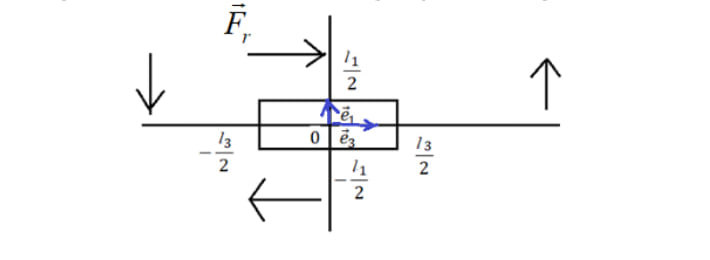
\includegraphics[width=0.7\linewidth]{semester8/img/27}
	\caption{}
	\label{fig:27}
\end{figure}

Пусть на боковых поверхностях $x_3 = \pm \frac{l_3}{2}$ и $x_1 = \pm \frac{l_1}{2}$ заданы касательные константы, вектор напряжений, а поверхность $x_2 = \pm \frac{l_2}{2}$ --- свободны. 

\begin{enumerate}
	\item На $x_1 = \pm \frac{l_1}{2}, \quad \mathbf{t}_{n_e} = \mathbf{n} \cdot \sigma = \tau \mathbf{b}_3 \quad (\sigma_{13} = \tau, \sigma_{12} = 0, \sigma_{11} = 0)$
		
	\item На $x_3 = \pm \frac{l_3}{2}, \quad \mathbf{t}_{n_e} = \mathbf{n} \cdot \sigma = \tau \mathbf{b}_1 \quad (\sigma_{13} = \tau, \sigma_{23} = 0, \sigma_{33} = 0)$
	
	\item На $x_2 = \pm \frac{l_2}{2}, \quad \mathbf{t}_{n_e} = \mathbf{n} \cdot \sigma = 0 \quad (\sigma_{12} = \tau, \sigma_{23} = 0, \sigma_{22} = 0)$
\end{enumerate}

Если массовых сил нет $\vec{f} = 0$ и процессы деформирования квазистатические, то напряжение, являющиеся решением и ГУ, имеет следующий вид:
\boxed{\sigma_{13} = \tau = \mathrm{const}}, а остальные \boxed{\sigma_{ij} \equiv 0} $\forall \vec{x} \in V$
\begin{itemize}
	\item Деформацию вычисляем:
	\begin{equation*}
		\varepsilon_{ij} = \Pi_{ijkl} \sigma_{kl} = 2 \Pi_{ij13} \tau
	\end{equation*}
	
	\item Для ортотропных сред:
	\begin{equation*}
		\varepsilon_{13} = 2 \Pi_{1313} \tau \Rightarrow \varepsilon_{13} = \frac{1}{2 G_{13} \tau}
	\end{equation*}
	
	\item Измеряя $\varepsilon_{13}$ и $\tau$ находим модуль сдвига. 
	\begin{equation*}
		\boxed{G_{13} = \frac{\tau}{2 \varepsilon_{13}}.}
	\end{equation*}
\end{itemize}

Для ортотропных сред задача о сдвиге используется для определения $G_{12}$, $G_{13}$ и $G_{23}$.

Для нахождения перемещений используем формулу Чезаро после жёсткого защемления одной точки, например, $\mathbf{x}_0 = 0$:
\begin{equation*}
	\boxed{\mathbf{u} = \varepsilon \cdot \mathbf{x}}, \quad \boxed{u_i = \varepsilon_{ij} \cdot x_{j}}
\end{equation*} 

\chapter{Основы механики жидкостей и газов}
\que{Модель газообразных сред: определяющие соотношения, замкнутая система уравнений для идеального газа в дивергентной форме и в полных дифференциалах. Уравнение движения в форме Громеки-Лемба}

\paragraph{Определение сплошных сред, определяющие соотношения для сплошных сред.}
\begin{definition}
  Сплошную среду, имеющую группу симметрий $\mathring{G}_s$ для любой отсчётной конфигурации
  $\mathring{\mathcal{K}}$, которая совпадает с полной унимодулярной группой
  $\mathring{G}_s = U$\footnote{\emph{полная унимодулярная группа} $U$ -- группа, состоящая из всех тензоров $H$, таких что $\det H = \pm 1$},
  называют \emph{жидкостью} (жидкой средой).
\end{definition}

Рассматривая различные модели сплошных сред, такие как $\overset{(n)}{A}$,
$\overset{(n)}{B}$, $\overset{(n)}{C}$, $\overset{(n)}{D}$, и применяя к ним принцип
материальной симметрии относительно полной унимодулярной группы, получим одни и те же
определяющие соотношения, т.о. все эти модели эквивалентны, а определяющие соотношения можно
представить в виде\footnote{подробнее см. Димитриенко 2 том, раздел 3.8.13, страница 304}:
\begin{equation}\label{eq:os_fluid_1}
  \begin{cases}
    T = - p E, \\
    p = p(\rho, \theta) = \rho^2 \dfrac{\partial \psi}{\partial \rho}, \\
    \psi = \Psi(\rho, \theta), \\
    \eta = - \dfrac{\partial \psi}{\partial \theta} 
  \end{cases}
\end{equation}

\paragraph{Замкнутая система уравнений для идеального газа в дивергентной форме.}

Уравнение неразрывности (никак не меняется от ОС):
\[
  \dfrac{\partial \rho}{\partial t} + \nabla \cdot (\rho \mathbf{v}) = 0.
\]

Уравнение движения (используем $T = - p E$):
\[
  \dfrac{\partial \rho\mathbf{v}}{\partial t} + \nabla \cdot \left( \rho \mathbf{v} \otimes \mathbf{v} + p E \right) = \rho \mathbf{f}.
\]

Уравнение для полной энергии (используем $T = -p E$, т.к. $\nabla \cdot (T \cdot\mathbf{v}) = - \nabla \cdot (p \mathbf{v}) = - \nabla \cdot (\rho \mathbf{v} (p / \rho)) $):
\[
  \dfrac{\partial \rho \varepsilon}{\partial t} + \nabla \cdot \left( \rho \mathbf{v} \dfrac{p}{\rho} + \mathbf{q} \right) = \rho \mathbf{f} \cdot \mathbf{v} + q_m,
\]
где $\varepsilon = e + \dfrac{\mathbf{v}^2}{2}$ -- полная энергия.

И добавляем определяющие соотношения \eqref{eq:os_fluid_1} в виде:
\[
  \begin{cases}
    p = p(\rho, \theta) = \rho^2 \dfrac{\partial \psi}{\partial \rho}, \\
    e = e(\rho, \theta) = \psi - \theta \dfrac{\partial \psi}{\partial \theta}, \\
    \psi = \psi(\rho, \theta).
  \end{cases}
\]
А также закон Фурье:
\[
  \mathbf{q} = - \lambda \nabla \theta.
\]

\paragraph{Замкнутая система уравнений для идеального газа в полных дифференциалах.}

Уравнение неразрывности:
\[
  \dfrac{d \rho}{dt} + \rho \nabla \cdot \mathbf{v} = 0.
\]
Уравнение движения (в такой форме его называют \emph{уравнением Эйлера}):
\[
  \rho \dfrac{d \mathbf{v}}{dt} = - \nabla p + \rho \mathbf{f}.
\]
Уравнение энергии:
\[
  \rho \dfrac{d\varepsilon}{dt} = - \nabla \cdot \left( p \mathbf{v} + \mathbf{q} \right) + \rho \mathbf{f} \cdot \mathbf{v} + \rho q_m.
\]
Определяющие соотношения остаются без изменений:
\[
  \begin{cases}
    p = p(\rho, \theta) = \rho^2 \dfrac{\partial \psi}{\partial \rho}, \\
    e = e(\rho, \theta) = \psi - \theta \dfrac{\partial \psi}{\partial \theta}, \\
    \psi = \psi(\rho, \theta), \\
    \mathbf{q} = - \lambda \nabla \theta.
  \end{cases}    
\]

\paragraph{Уравнение движения в форме Громеки-Лемба.}

\begin{theorem}
  Уравнение движения Эйлера всегда можно представить в форме Громеки-Лемба:
  \[
    \dfrac{\partial \mathbf{v}}{\partial t} + \nabla \dfrac{|\mathbf{v}|^2}{2} + 2 \mathbf{\omega} \times \mathbf{v} = - \dfrac{1}{\rho} \nabla p + \mathbf{f},
  \]
  где $\mathbf{\omega} = \dfrac{1}{2} \nabla \times \mathbf{v}$ -- вектор вихря.
\end{theorem}

\paragraph{+ Другой вид уравнения энергии.}
Выведем теперь другой вид уравнения энергии из уравнения относительно $\varepsilon$ в полных
дифференциалах. Для начала получим \emph{теорему живых сил}, которая получается путём домножения
уравнения движения Эйлера скалярно на $\mathbf{v}$, а далее путём пары преобразований можно
получить:
\[
  \rho \dfrac{d}{dt} \left( \dfrac{|\mathbf{v}|^2}{2} \right) = - \mathbf{v} \cdot \nabla p + \rho \mathbf{f} \cdot \mathbf{v}.
\]

Теперь вычтем это уравнение из уравнения энергии в полных дифференциалах, учитывая, что $\varepsilon = e + |\mathbf{v}|^2/2$:
\begin{equation}\label{eq:fluid_energy_2}
  \rho \dfrac{de}{dt} = - p \nabla \mathbf{v} - \nabla \cdot \mathbf{q} + \rho q_m.
\end{equation}

\que{Модель совершенного газа, термодинамические функции. Модель совершенного газа с постоянными теплоемкостями.}


\que{Модель идеальной несжимаемой жидкости.}

\begin{definition}
  Сплошную среду называют \emph{несжимаемой}, если в любой актуальной конфигурации $\mathcal{K}$
  её плотность $\rho$ совпадает с плотностью $\mathring{\rho}$ в отсчётной конфигурации:
  \[
    \rho = \mathring{\rho} = \operatorname{const}, \forall t \geqslant 0, \forall \mathcal{K}
  \]
\end{definition}

Из уравнения неразрывности в переменных Лагранжа следует, что для несжимаемых сред объём любого
элементарного параллелепипеда $dV$ не изменяется:
\[
  \rho = \mathring{\rho} \Rightarrow dV = d\mathring{V},
\]
а, следовательно, и объём $|V(t)|$ области, которую занимает несжимаемая среда, не изменяется:
$|V(t)| = |\mathring{V}| = \operatorname{const}$.

Из уравнения неразрывности следует также, что для несжимаемой среды всегда существует
дополнительное условие на градиент деформации:
\[
  \det F = 1.
\]

Используя полярное разложение, находим, что для несжимаемой среды тензоры искажений всегда имеют 
единичный детерминант:
\[
  \det V = \det F \cdot \det O^T = \det F = 1, \quad \det U = 1.
\]
Тогда, находим, что детерминант всех энергетических и квазиэнергетических мер деформации тоже
всегда имеет постоянное значение:
\begin{align*}
  \det \overset{(n)}{G} &= \det \left( \dfrac{1}{n - III} U^{n - III} \right) = 
  \dfrac{1}{(n-III)^3} \det U^{n - III} = \dfrac{1}{(n-III)^3}, \\
  \det \overset{(n)}{g} &= \det \left( \dfrac{1}{n - III} V^{n - III} \right) = 
  \dfrac{1}{(n-III)^3}, \quad n = I, II, III, IV, V.
\end{align*}

Уравнение неразрывности для несжимаемой жидкости (т.н. \emph{уравнение несжимаемости}):
\[
  \nabla \cdot \mathbf{v} = 0.
\]
Уравнение движения для несжимаемой жидкости:
\[
  \dfrac{\partial \mathbf{v}}{\partial t} + \nabla \cdot \left( \mathbf{v} \otimes \mathbf{v} + \dfrac{p}{\rho} E \right) = \mathbf{f}.
\]
Уравнение энергии для несжимаемой жидкости:
\[
  \dfrac{\partial \varepsilon}{\partial t} + \nabla \cdot \left( \mathbf{v}\cdot \left( \varepsilon+\dfrac{p}{\rho} \right) + \dfrac{\mathbf{q}}{\rho} \right) = \mathbf{f}\cdot\mathbf{v} + q_m.
\]

Определяющие соотношения для несжимаемой жидкости:
\[
  \begin{cases}
    \varepsilon = e + \dfrac{|\mathbf{v}|^2}{2}, \\
    e = \psi + \theta \eta = \psi - \theta \dfrac{\partial \psi}{\partial \theta} = e(\theta), \\
    \psi = \psi(\rho, \theta) = \psi(\theta), \\
    \mathbf{q} = - \lambda \nabla \theta
  \end{cases}
\]
Определяющее соотношение $p = \rho^2 \dfrac{\partial \psi}{\partial \rho}$ пропадает, а
давление становится самостоятельной независимой функцией.

% \paragraph{Модель совершенной несжимаемой жидкости.}


\que{Соотношения на поверхностях сильных разрывов в идеальных газах. Соотношения Гюгонио.}


\que{Соотношения на поверхности разрыва в идеальном газе без перехода материальных точек через поверхность}

Соотношения Гюгонио были установлены для случая $M \not = 0$, т.е. при наличии перехода материальных точек через поверхность $S(t)$ (случай ударных волн и фазовых превращений). 

Если материальные точки не переходят через поверхность $S(t)$, то $M = 0$ и из соотношений из теоремы из предыдущего вопроса \ref{3} следует, что:
\begin{equation*}
	-M = \rho_1 u_1 = \rho_1 \left(v_{n_1} - D\right) = \rho_2 \left(v_{n_2} - D\right) = 0.
\end{equation*}

Поскольку $\rho_1 \not = 0$ и $\rho_2 \not = 0$, то нормальные составляюзие скорости при переходе через $S$ являются непрерывными:
\begin{equation*}
	M = 0, \quad v_{n_1} = v_{n_2} = D, \quad u_1 = u_2 = 0.
\end{equation*}

Тогда находим:
\begin{equation*}
	p_1 - p_2 = C_{n\Sigma}.
\end{equation*}

Если поверхностные усилия отсутствуют: $C_{n\Sigma} = 0$, то давление при переходе через $S(t)$ также остается непрерывными:
\begin{equation*}
	p_1 = p_2.
\end{equation*}

Третье соотношение, все той же системы, в случае $M = 0$ сводится к простому условию:
\begin{equation*}
	C'_{3\Sigma} - C_{n\Sigma} D = 0,
\end{equation*}
или
\begin{equation*}
	q_{n_1} - q_{n_2} = C_{3\Sigma} - D C_{n\Sigma}.
\end{equation*}

Если поверхностные усилия и энергия отсутствуют: $C_{3\Sigma} = -. C_{n\Sigma} = 0$, то получаем условие непрерывности нормальной составляющей теплового потока:
\begin{equation*}
	q_{n_1} = q_{n_2}.
\end{equation*}
Таким образом, доказана следующая теорема.

\begin{theorem}
	В случае отсутствия перехода материальных точек черех поверхность разрыва $S(t)$ в идеальном газе давление $p$, нормальные составляющие скорости $v_n$ и теплового потока $q_n$ остаются непрерывными при переходе через $S$, остальные же функции $v_{\tau_\alpha}$, $e$, $\theta$ и $\rho$ могут терпеть разрыв. 
\end{theorem}
\que{Соотношения на поверхности разрыва идеальной газовой и твердой сред.}

% TODO: \usepackage{graphicx} required
\begin{figure}[h!]
	\centering
	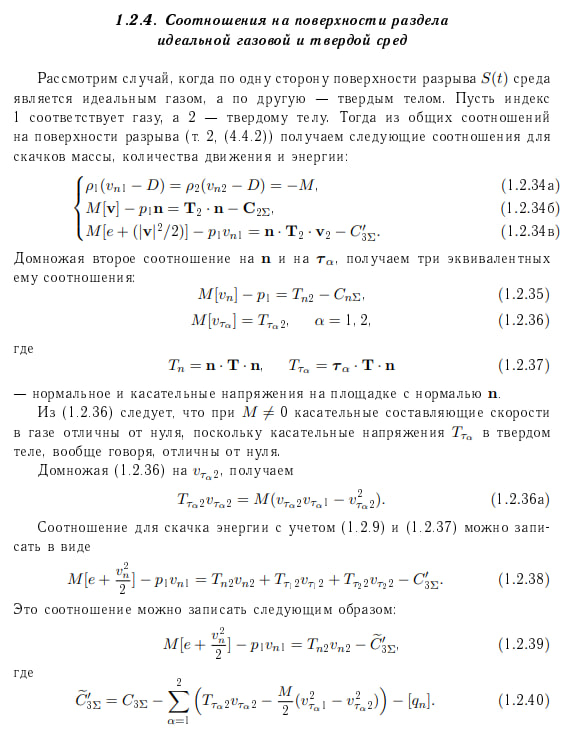
\includegraphics[width=0.9\linewidth]{semester8/img/33_1}
\end{figure}

% TODO: \usepackage{graphicx} required
\begin{figure}[h!]
	\centering
	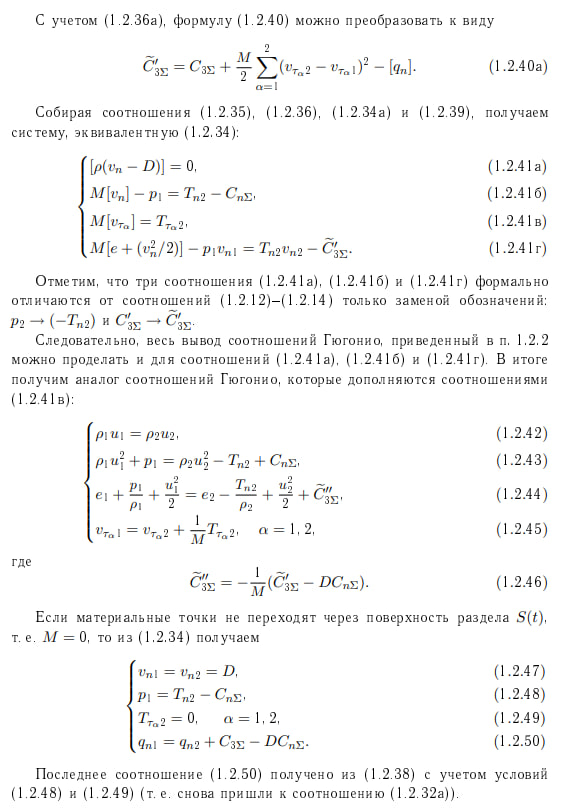
\includegraphics[width=0.9\linewidth]{semester8/img/33_2}
\end{figure}

% TODO: \usepackage{graphicx} required
\begin{figure}[H]
	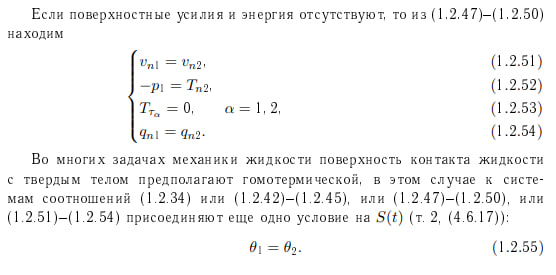
\includegraphics[width=0.9\linewidth]{semester8/img/33_3}
\end{figure}



\que{Адиабатические процессы в идеальных газах. Адиабата Пуассона. }

\begin{definition}
  Если в уравнениях движения и энергии идеального газа (жидкости) можно пренебречь членами,
  связанными с массовыми и поверхностными притоками тепла, т.е. $q_m = 0, \mathbf{q} = 0$,
  то говорят, что рассматривается \emph{модель адиабатических процессов в идеальной жидкости
  или газе}.
\end{definition}

% **Следствие из адиабатичности.**

\paragraph{Адиабата Пуассона.}

Рассмотри уравнение баланса энтропии для идеальной жидкости:
\[
  \rho \theta \dfrac{d\eta}{dt} = - \nabla\cdot\mathbf{q} + \rho q_m + w^*,
\]
в котором $w^* = 0$, т.к. жидкость идеальная.
Тогда для адиабатических процессов:
\[
  \rho\theta \dfrac{d\eta}{dt} = 0.
\]
Так как по определению $\rho > 0$ и $\theta > 0$, то
\[
  \dfrac{d\eta}{dt} = 0
\]
в этом выражении $\eta = \eta(x^i, t)$, перейдём к лагранжевому описанию, в котором
$\eta(x^i, t) = \tilde \eta(X^i, t)$. Полная производная $\dfrac{d}{dt}$ расписывается как
\[
  \dfrac{d\eta}{dt} = \dfrac{\partial \eta}{\partial t} + \mathbf{v} \cdot \nabla \eta =
  \dfrac{\partial \tilde \eta (X^i, t)}{\partial t} = 0
\]
тогда:
\[
  \eta(X^i, t) = \mathring{\eta}(X^i)
\]
-- \emph{адиабата Пуассона} в наиболее общем виде.

\paragraph{Физический смысл адиабаты Пуассона.}
Плотность энтропии каждой материальной точки вдоль её траектории не меняется. Поэтому адиабатические процессы также называют \emph{иээнтропическими}.


Вспоминая определяющие соотношения, можно получить соотношение между плотностью и температурой каждой материальной точки:
\[
  \eta = - \dfrac{\partial \psi}{\partial \theta} =
  \eta \left(\rho(X^i, t), \theta(X^i, t) \right) = \mathring{\eta}(X^i).
\]
% -- адибата Пуассона в общем виде.

\que{Адиабата Пуассона для совершенного газа.}

\paragraph{Адиабата Пуассона для совершенного газа.}
В выражении для $\eta$ в совершенном газе обозначим:
\[
  \eta\left(\rho(X^i, t), \theta(X^i, t)\right) =
  - \dfrac{\partial \psi}{\partial \theta}  =
  \eta_0 +
  % \int\limits_{\theta_0}^\theta C_v(\tilde\theta) \, d\tilde\theta +
  \underbrace{\int\limits_{\theta_0} \dfrac{c_v(\tilde \theta)}{\tilde \theta} \, d\tilde \theta + R \ln \dfrac{\rho_0}{\rho}}_{\Delta \eta} =
  \eta_0 + \Delta \eta =
  \mathring{\eta}(X^i)
\]
т.е.
\[
  \int\limits_{\theta_0} \dfrac{c_v(\tilde \theta)}{\tilde \theta} \, d\tilde \theta + R \ln \dfrac{\rho_0}{\rho} =
  \eta - \Delta \eta =
  \operatorname{const}
\]

\paragraph{Для модели совершенного газа с постоянной теплоёмкостью.}
Если теперь $c_v = \operatorname{const}$, то интегралы в последнем выражении можно найти
и получить
\[
  c_v \ln \dfrac{\theta}{\theta_0} = R \ln \dfrac{\rho}{\rho_0} + \Delta \eta,
\]
или
\[
  \dfrac{\theta}{\theta_0} = e^{\dfrac{\Delta \eta}{c_v}} \left(\dfrac{\rho}{\rho_0}\right)^{\dfrac{R}{c_v}}
\]
обозначая в последнем $A_0 = e^{\dfrac{\Delta\eta}{c_v}}$; вспоминая коэффициент Пуассона $k = \dfrac{c_p}{c_v} = \dfrac{c_v + R}{c_v}$, получаем
\begin{equation}\label{eq:poisson_adiabata_0}
  \dfrac{\theta}{\theta_0} = A_0 \left( \dfrac{\rho}{\rho_0} \right)^{k-1}
\end{equation}
-- адиабата Пуассона для идеального совершенного газа с постоянными теплоёмкостями
в форме $\theta \sim \rho$.

\textit{Другие формы адиабаты Пуассона для совершенного газа с постоянными теплоёмкостями.}

Отметим, что адиабата Пуассона \eqref{eq:poisson_adiabata_0} содержит параметры газа
$\theta_0, \rho_0, \eta_0$ -- табличные значения в некотором известном (<<начальном>>) состоянии.
Получим теперь это же соотношение, считая известными параметры газа в некоторой конфигурации
$\mathcal{K}_1$, в которой газ имеет параметры $\theta_1, \rho_1, \eta_1$. Запишем адиабату
Пуассона два раза: для известного состояния $\mathcal{K}_1$ и для некоторой произвольной
конфигурации $\mathcal{K}$:
\[
  \begin{cases}
    \dfrac{\theta_1}{\theta_0} = A_0 \left( \dfrac{\rho_1}{\rho_0} \right)^{k-1} \\
    \dfrac{\theta}{\theta_0} = A_0 \left( \dfrac{\rho}{\rho_0} \right)^{k-1}
  \end{cases}
\]
поделим второе выражение на первое и получим
\begin{equation}\label{eq:poisson_adiabata_1}
  \dfrac{\theta}{\theta_1} = \left( \dfrac{\rho}{\rho_1} \right)^{k-1}
\end{equation}
-- адиабата Пуассона для совершенного газа с постоянными теплоёмкостями, выраженная через
некоторую конфигурацию $\mathcal{K}_1$.

\textit{Адиабата Пуассона в форме $p \sim \rho$}
Из соотношения Менделеева-Клапейрона $p = \rho R \theta$ выразим температуру $\theta = \dfrac{p}{\rho R}$, тогда адиабата Пуассона \eqref{eq:poisson_adiabata_1} принимает вид:
\[
  \dfrac{p \rho_1 R}{p_1 \rho R} = \left(\dfrac{\rho}{\rho_1} \right)^{k-1},
\]
сокращая всё что можно сократить, получаем
\begin{equation}\label{eq:poisson_adiabata_2}
  \dfrac{p}{p_1} = \left( \dfrac{\rho}{\rho_1} \right)^{k}
\end{equation}
-- ещё одна адиабата Пуассона.

Её ещё можно преобразовать, введя $A = \dfrac{p_1}{\rho_1^k}$, к виду
\begin{equation}\label{eq:poisson_adiabata_3}
  p = A \rho^k
\end{equation}

Ещё можно ввести \emph{удельный объём} $V = \dfrac{1}{\rho}$, тогда
\begin{equation}\label{eq:poisson_adiabata_2}
  \dfrac{p}{p_1} = \left( \dfrac{V_1}{V} \right)^{k}
\end{equation}

\paragraph{Внутренняя энергия совершенного идеального газа с постоянными теплоёмкостями.}
Для совершенного газа было получено:
\[
  e = e_0 + c_v(\theta - \theta_0) = \tilde e_0 + c_v \theta
\]
используя соотношение Менделеева-Клапейрона в виде $\theta = \dfrac{p}{\rho R}$ получаем:
\[
  e = \tilde e_0 + \dfrac{c_v p}{\rho R} = \tilde e_0 + \dfrac{p}{\rho (k-1)} =
  \tilde e_0 + \dfrac{pV}{k-1}
\]

\que{Система уравнений газовой динамики для адиабатических процессов.}

% TODO
(видимо имеется ввиду адиабатические процессы в совершенном газе, если газ не совершенный,
то я информации не нашёл)


Уравнение энергии можно исключить из общей системы уравнений в идеальном совершенном газе,
поэтому замкнутая система будет выглядеть так:
\[
  \begin{cases}
    \dfrac{\partial \rho}{\partial t} + \nabla \cdot (\rho \mathbf{v}) = 0, \\
    \dfrac{\partial \mathbf{v}}{\partial t} + \mathbf{v} \cdot \nabla \otimes \mathbf{v} = - \dfrac{1}{\rho} \nabla p + \mathbf{f}, \\
    p = A \rho^k, \quad A = \dfrac{\mathring{p}}{\mathring{\rho}^k}
  \end{cases}
\]

\que{Соотношения Гюгонио для адиабатических процессов в совершенном газе.}

Пусть в совершенном газе есть поверхность разрыва, до разрыва газ
имеет макроскопические характеристики $\rho_1, p_1, u_1$, после разрыва -- $\rho_2, p_2, u_2$
(по обе стороны от разрыва находится одинаковый газ),
тогда соотношения Гюгонио:
\[
  \begin{cases}
    \rho_1 u_1 = \rho_2 u_2, \\
    \rho_1 u_1^2 + p_1 = \rho_2 u_2^2 + p_2, \\
    \dfrac{k}{k-1} \dfrac{p_1}{\rho_1} + \dfrac{u_1^2}{2} = \dfrac{k}{k-1} \dfrac{p_2}{\rho_2} + \dfrac{u_2^2}{2}.
  \end{cases}
\]
% Пусть $\mathbf{D}$ -- скорость движения поверхности разрыва.

Найдём значения $\rho_1, p_1, u_1$ при известных $\rho_2, p_2, u_2$.

Обозначим $\gamma = \dfrac{\rho_2}{\rho_1}$, тогда
\[
  \begin{cases}
    u_1 = \gamma u_2, \\
    p_1 = p_2 + \rho_2 u_2^2 (1 - \gamma), \\
    \dfrac{k}{k-1} \dfrac{\rho_2}{\rho_1} u_2^2 (1 - \gamma) + \dfrac{k}{k-1} \dfrac{p_2}{\rho_1} \dfrac{\rho_2}{\rho_2} + \dfrac{\gamma^2 u_2^2}{2} - \dfrac{k}{k-1} \dfrac{p_2}{\rho_2} - \dfrac{u_2^2}{2} = 0
  \end{cases}
\]
преобразуем последнее выражение к виду:
\[
 \gamma(1-\gamma) + (\gamma^2 - 1) \dfrac{k-1}{2k}+ \dfrac{p_2}{u_2^2 \rho_2} (\gamma-1) = 0
\]
или (обозначили $B = \dfrac{p_2}{\rho_2 u_2^2}$)
\[
  \gamma^2 - \dfrac{2k}{k+1} (1 + B) \gamma + \dfrac{k-1}{k+1} = 0
\]
тогда
\[
  \gamma_{1, 2} = \dfrac{1}{1+k} \left( k(1+B) \pm (1 - kB) \right)
  \Leftrightarrow
  \gamma_1 = \dfrac{k-1 +2kB}{k+1}, \; \gamma_2 = 1,
\]
случай $\gamma = 1$ не рассматриваем, т.к. в этом случае никакого разрыва нет (можно проверить,
что тогда $\rho_1=\rho_2, u_1=u_2, p_1=p_2$ из соотношений Гюгонио).

Таким образом, при адиабатических процессах в совершенном газе с постоянными теплоёмкостями
и при отсутствии поверхностных эффектов на поверхности разрыва соотношения Гюгонио принимают вид:
\[
  \begin{cases}
    \dfrac{1}{\rho_1} = \dfrac{k-1}{k+1}\dfrac{1}{\rho_2} + \dfrac{2k}{k+1} \dfrac{p_2}{\rho_2^2 u_2^2}, \\
    p_1 = \dfrac{2}{k+1} \rho_2 u_2^2 - \dfrac{k-1}{k+1} p_2, \\
    u_1 = \dfrac{k-1}{k+1} u_2 + \dfrac{2k}{k+1} \dfrac{p_2}{\rho_2 u_2}.
  \end{cases}  
\]

\que{Адиабата Гюгонио и луч Михельсона.}

Пусть в совершенном газе есть поверхность разрыва, до разрыва газ
имеет макроскопические характеристики $\rho_1, p_1, u_1, e_1$, после разрыва -- $\rho_2, p_2, u_2, e_2$
(по обе стороны от разрыва находится одинаковый газ с одинаковыми определяющими соотношениями),
при этом материальные точки \textit{переходят} через поверхность разрыва: $M = \mathbf{D} \rho \neq 0$, где $\mathbf{D}$ -- скорость этой поверхности. 
Такую поверхность называют поверхностью ударной волны.

Положим $C_{n\Sigma} = C_{3\Sigma} = 0$, введём удельные объёмы
$V_1 = 1 / \rho_1, V_2 = 1 / \rho_2$. Тогда соотношения Гюгонио можно записать в виде:
\[
  \begin{cases}
    \dfrac{u_1}{V_1} = \dfrac{u_2}{V_2}, \\
    \dfrac{u_1^2}{V_1} - \dfrac{u_2^2}{V_2} = p_2 - p_1, \\
    e_1 - e_2 = \dfrac{u_2^2 - u_1^2}{2} + p_2 V_2 - p_1 V_1.
  \end{cases}
\]
Пусть значения после разрыва будут известными, тогда выразим значения до разрыва:
\[
  \begin{cases}
    u_1 = \dfrac{V_1 u_2}{V_2}, \\
    u_2^2 \dfrac{V_1}{V_2^2} - \dfrac{u_2^2}{V_2} = p_2 - p_1 \Rightarrow \dfrac{u_2^2}{V_2^2} = \dfrac{p_2-p_1}{V_1 - V_2},
  \end{cases}
\]
тогда
\[
  \begin{cases}
    u_2 = \pm V_2 \sqrt{\dfrac{p_2-p_1}{V_1 - V_2}}, \\
    u_1 = \pm V_1 \sqrt{\dfrac{p_2 - p_1}{V_1 - V_2}}
  \end{cases}
\]
найдём тогда скачок внутренней энергии:
\[
  [e] = e_2 - e_1 = p_1 V_1 - p_2V_2 + \dfrac{u_1^2 - u_2^2}{2} =
  \dfrac{p_2-p_1}{V_1-V_2} \dfrac{V_1^2 - V_2^2}{2} + p_1V_1 - p_2V_2 =
  \dfrac{1}{2} (p_1+p_2) (V_1 - V_2)
\]
полученное выражение называется \emph{адиабатой Гюгонио} (или \emph{ударной адиабатой}).

Если известны $e_i (p_i, V_i)$, то адиабата Гюгонио связывает между собой давление и удельный
объём с одной и с другой стороны поверхности раздела, т.е. если с одной из сторон разрыва
газ принимает значения $(p_1, V_1)$, то с другой стороны газ может принимать множество разных
значений $(p_2, V_2)$, но обязательно лежащих на этой кривой.

\paragraph{Адиабата Гюгонио для совершенного газа.}
Стоит отметить, что в случае совершенного газа $e = \tilde e_0 + \dfrac{pV}{k-1}$,
тогда в случае совершенного газа (пусть нет скачка начальной внутренней энергии $\tilde e_0$):
\[
  \dfrac{p_2V_2 - p_1V_1}{k-1} = \dfrac{1}{2} (p_1+p_2) (V_1 - V_2).
\]
\begin{figure}[H]
  \centering
  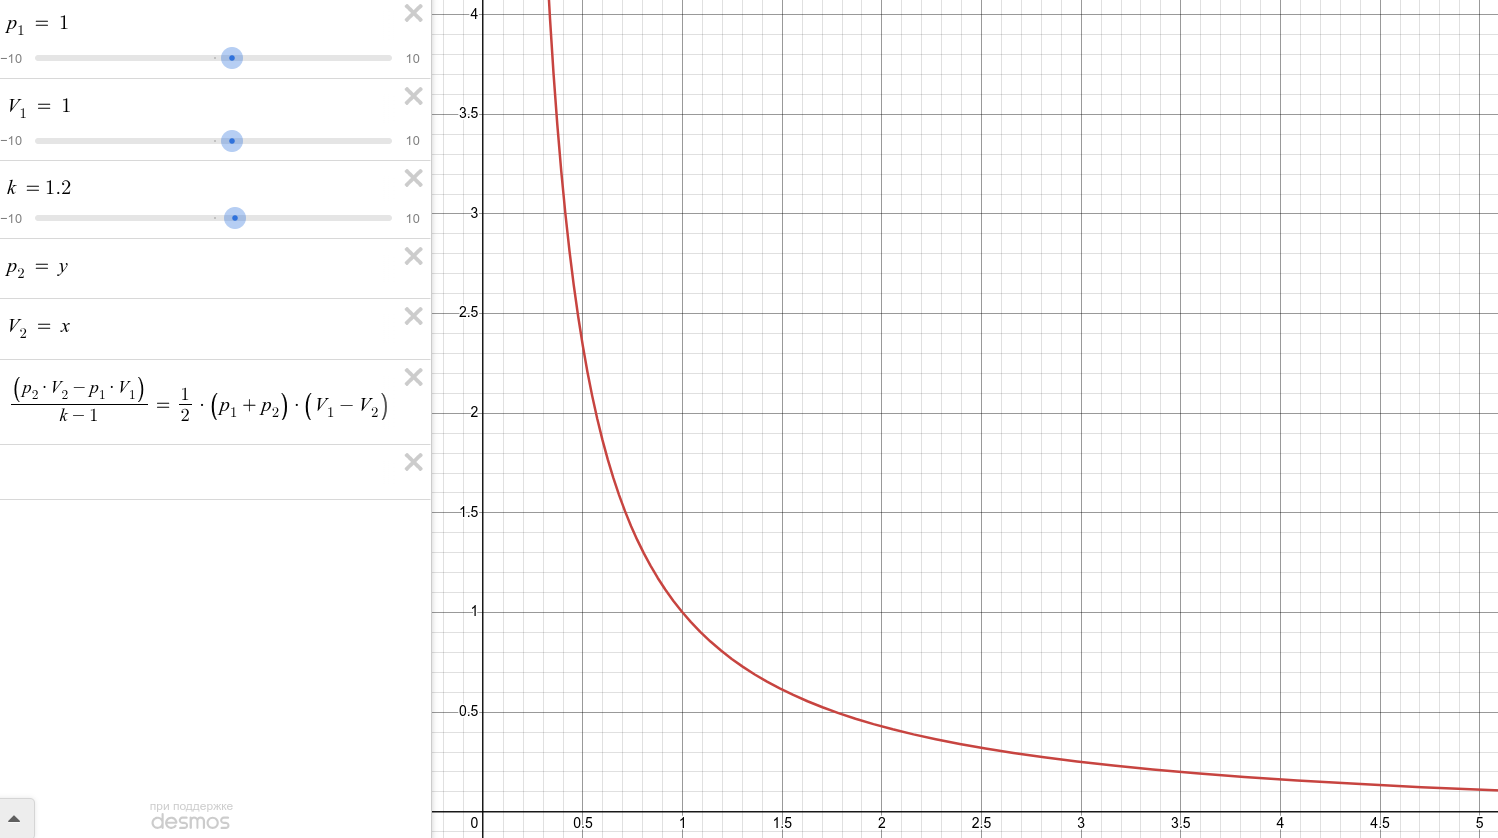
\includegraphics[width=0.9\linewidth]{img/Gugonio_adiabata_desmos.png}
  \caption{Адиабата Гюгонио для совершенного газа при адиабатических процессах. Фото в цвете}
\end{figure}

\paragraph{Доказательство невозрастания.}
Адиабата Гюгонио всегда (при любых фиксированных $(p_1, V_1)$) невозрастает. 
\begin{proof}
  Для доказательства этого покажем, что любая секущая, проходящая через
  точку $(p_1, V_1)$ и точку $(p_2, V_2)$ невозрастает.
  Уравнение секущей: $p - p_1 = \tg \alpha \cdot (V - V_1)$, 
  а $\tg \alpha$ можно найти из выражения для $u_2 = \pm V_2 \sqrt{\dfrac{p_2-p_1}{V_1 - V_2}}$:
  \[
    \tg \alpha  = \dfrac{p_2 - p_1}{V_2 - V_1} = - \dfrac{u_2^2}{V_2} \leqslant 0
  \]
  Таким образом, любая секущая невозрастает, а значит и сама адиабата невозрастает.
\end{proof}

Построенная секущая называется \emph{лучом Михельсона} (также Релея) (луч, потому что $p \geqslant 0$).

\que{Cвойства адиабаты Гюгонио.}


\que{Взаимное  расположение  адиабат  Гюгонио  и  Пуассона  в  идеальном  газе.  Адиабата  Гюгонио  для совершенного газа.}


\que{Плоские волны в газовой динамике. Автомодельное решение одномерной задачи газовой динамики.}


\que{Характеристические направления в одномерной задаче, инварианты Римана, решение Римана.}


\que{Задача о поршне, выдвигаемом из газа.}


\que{Определение квазистатических процессов в жидкостях. Закон Паскаля. Задача о равновесии жидкости в поле силы тяжести.}

\begin{definition}
  Если в системе уравнений МЖГ для идеальной сжимаемой жидкости или в системе для несжимаемой
  жидкости пренебрегают членами, содержащими скорость $\mathbf{v}$, т.е. полагают
  $\mathbf{v} \equiv 0$, то говорят, что принята модель \emph{квазистатических процессов в
  жидкости}.
\end{definition}

В таком случае идеальная сжимаемая жидкость удовлетворяет уравнениям
\[
  \begin{cases}
    \dfrac{\partial \rho}{\partial t} = 0, \\
    \nabla p = \rho \mathbf{f}, \\
    \rho \dfrac{\partial e}{\partial t} + \nabla \cdot \mathbf{q} = \rho q_m.
  \end{cases}
\]
Второе уравнение этой системы называют \emph{уравнением равновесия жидкости}.

\paragraph{Закон Паскаля.} Если внешние массовые силы отсутствуют, то при квазистатических
процессах уравнение равновесия принимает вид $\nabla p = 0$, то есть давление $p = p(t)$ --
не зависит от координат и одинаково для всех точек в данный момент времени.
Это называют \emph{законом Паскаля}.

\paragraph{Задача о равновесии жидкости в поле силы тяжести.} 
Рассмотрим следующую задачу: пусть жидкость находится в равновесии в поле силы тяжести
$\mathbf{f}$.
Так как рассматриваем небольшой участок планеты, то будем считать ускорение свободного падения
постоянным и равным $g_\Sigma$ (для Земли оно примерно равно $9.8 \text{м}/\text{с}^2$). 
Декартову систему координат введём таким образом, чтобы ось $\bar{\mathbf{e}}_3$ была направлена
вверх, соответственно в такой системе координат $\mathbf{f} = - g_\Sigma \bar{\mathbf{e}}_e$,
тогда условие равновесия можно расписать покомпонентно:
\[
  \begin{cases}
    \dfrac{\partial p}{\partial x^1} = \dfrac{\partial p}{\partial x^2} = 0, \\
    \dfrac{\partial p}{\partial x^3} = - \rho g_\Sigma = - \dfrac{p g_\Sigma}{R\theta},
  \end{cases}
\]
(здесь использовано соотношение Менделеева-Клапейрона $\rho = p/(R\theta)$).

Решением этого уравнения будет являтся так называемая \emph{барометрическая формула}:
\[
  p = p_0 \exp \left( - \int\limits_{x^3_0}^{x^3} \dfrac{g_\Sigma \, dx}{R\theta} \right),
\]
где $p_0$ -- давление при $x^3 = x^3_0$.

Третье уравнение системы для квазистатических процессов в совершенном газе перепишем в виде:
\[
  \rho c_v \dfrac{\partial \theta}{\partial t} = \lambda \Delta \theta + \rho q_m,
\]
которое называется \emph{уравнением теплопроводности для совершенного газа в состоянии
равновесия}.

Если процесс распространения тепла в газе является стационарным (установившимся), т.е. 
$\partial \theta / \partial t = 0$, то получаем стационарное уравнение теплопроводности:
\[
  \Delta \theta + \dfrac{pq_m}{\lambda R \theta} = 0.
\]



\que{Задача о равновесии стандартной атмосферы.}

Рассматривается задача о равновесии в поле силы тяжести на высотах
$0 \leqslant z = x^3 - x_0^3 \leqslant H$, как в прошлом вопросе,
в которой плотность внешних массовых сил $\mathbf{f} = - g_\Sigma \bar{\mathbf{e}}_3$,
при этом для нахождения давления предполагают, что температура равна некоторой константе
$\bar{\theta}$, тогда используя барометрическую формулу (см. предыдущий вопрос):
\[
  p = p_0 \exp \left( - \int\limits_0^z \dfrac{g_\Sigma \, dx}{R \bar{\theta}} \right) =
  p_0 \exp \left( - \beta_0 z \right), \quad \beta_0 = \dfrac{g_\Sigma}{R\bar{\theta}}, \quad
  \rho = \rho_0 \exp \left( - \beta_0 z \right).
\]

Теперь найдём стационарное распределение температуры от высоты. Для этого необходимо
определить чему равна плотность внешних массовых источников тепла $q_m$, которая
в реальности в основном определяется поглощением излучения атмосферы. 
Зададим эту плотность кусочно-постоянной, т.е. разобьём $[0, H]$ на подотрезки
$[H_i, H_{i+1}], i = 0, 1, \dots, n-1$, где $0 = H_0 < H_1 < \dots < H_n = H$.
На каждом таком подотрезке $q_m = q_{mi}, z \in [H_i, H_{i+1}]$. Найдём температуру из 
стационарного уранвнения теплопроводности:
\[
  \dfrac{d^2\theta}{dz^2} + \dfrac{\rho q_m}{\lambda} = 0
  \Leftrightarrow
  \dfrac{d^2 \theta}{dz^2} = - \dfrac{q_m \rho_0}{\lambda} \exp \left( - \beta_0 z \right),
\]
тогда решение будет представляться в виде:
\[
  \theta = \theta^{(i)} = - \dfrac{\rho_0 q_{mi}}{\lambda \beta_0^2} \exp \left( - \beta_0 z \right) + a_i z + b_i, \; z \in [H_i, H_{i+1}],
\]
а коэффициенты $a_i, b_i$ будут определяться из условий непрерывности $\theta$ и
$\partial \theta / \partial z$ в точках $H_i$, а также из граничных условий $\theta(0) = \theta_0$,
$\theta(H) = \theta_H$.

\que{Установившиеся процессы в идеальных газах. Функция давления, выражения для нее при адиабатических процессах в совершенном газе (3 формы). Функция давления для несжимаемой жидкости.}

\begin{definition}
  Если для идеальной жидкости (как сжимаемой, так и несжимаемой) принимают допущение, 
  что функции $\mathbf{v}, p, \rho, \theta$ зависят только от координат, но не от времени, то
  говорят, что принята модель \emph{установившихся} (или \emph{стационарных}) процессов в
  жидкости.
\end{definition}

Для сжимаемой жидкости система уравнений МЖГ при установившихся процессах принимает вид:
\[
  \begin{cases}
    \nabla \cdot (\rho \mathbf{v}) = 0, \\
    \nabla \cdot \left( \rho \mathbf{v} \otimes \mathbf{v} + p E \right) = \rho \mathbf{f}, \\
    \nabla \cdot \left( \rho \mathbf{v} (\varepsilon + \dfrac{p}{\rho}) + \mathbf{q} \right) = \rho \mathbf{f} \cdot \mathbf{v} + \rho q_m.
  \end{cases}
\]

Для несжимаемой:
\[
  \begin{cases}
    \nabla \cdot \mathbf{v} = 0, \\
    \nabla \cdot \left( \mathbf{v} \otimes \mathbf{v} + \dfrac{p}{\mathring{\rho}} E \right) = \mathbf{f}, \\
    \nabla \cdot \left( \mathbf{v} \left( \varepsilon + \dfrac{p}{\mathring{\rho}} \right) + \mathbf{q} \right) = \mathbf{f} \cdot \mathbf{v} + q_m.
  \end{cases}
\]

Эти системы допускают существования первого интеграла, если ввести т.н. \emph{функцию давления}.

\paragraph{Функция давления.}
Пусть есть некоторая несамопересекающаяся кривая $\mathcal{L}$, которая проходит через
точку $\mathcal{M}_1 ( x^i_1 )$ и имеет уравнение
$x^i = x^i_\mathcal{L} (x^j_1, \tau), \tau \in [\tau_1, \tau_2]$. Тогда в установившемся
процессе, когда $\rho$ и $p$ являются функциями только координат, можно найти их как
зависимости от $\tau$: $\rho = \rho(x^i(x^j_1, \tau)) = \rho(\tau, \mathcal{L})$,
$p = p(x^i(x^j_1, \tau)) = p(\tau, \mathcal{L})$, тогда если эти зависимости взаимнооднозначные,
то можно построить зависимость $\rho = \rho(p, \mathcal{L})$.

Введём \emph{функцию давления} $\mathcal{P} (p, \mathcal{L})$:
\[
  \mathcal{P} (p, \mathcal{L}) = \int\limits^p \dfrac{dp'}{\rho(p', \mathcal{L})}
  \Leftrightarrow
  \dfrac{d\mathcal{P}}{dp} = \dfrac{1}{\rho(p, \mathcal{L})},
\]
где нижний предел не важен.

Можно доказать следующую теорему:
\begin{theorem}\footnote{эта теорема не до конца сформулирована в третьем томе Димитриенко}
  В баротропной в шикором смысле жидкости при установившихся процессах 
  функция давления не зависит от кривой $\mathcal{L}$, а только от значения давления
  и плотности в точке $\mathcal{M}_1$:
  \[
    \mathcal{P}(p, \mathcal{L}) = \mathcal{P}(p, \rho_1, p_1) = \int\limits^p \dfrac{dp'}{\rho(p, \rho_1, p_1)}
  \]
\end{theorem}

\paragraph{Функция давления при абиабатических процессах в совершенном газе.}
При адиабатических процессах в совершенном газе с постоянными теплоёмкостями (которые
являются баротропными в широком смысле) функция давления может быть найдена:
\[
  \mathcal{P}(p, \rho_1, p_1) = \int\limtis^p \left( \dfrac{p'}{p_1} \right)^{- 1/k} \dfrac{dp'}{\rho_1} = \dfrac{p_1}{\rho_1} \dfrac{k}{k-1} \left( \dfrac{p}{p_1} \right)^{(k-1)/k} =
  c_p \theta_1 \left( \dfrac{p}{p_1} \right)^{(k-1)/k}
\]

Другие формы для функции давления при адиабатических процессах в совершенном газе:
воспользуемся соотношением Мендлеева-Клапейрона $p / p_1 = \left( \rho / \rho_1 \right)^k $,
тогда:
\[
  \mathcal{P} = \dfrac{p_1}{\rho_1} \dfrac{k}{k-1} \left( \dfrac{\rho}{\rho_1} \right)^{k-1} =
  c_p \theta_1 \left( \dfrac{\rho}{\rho_1} \right)^{k-1},
\]
так как $p / p_1 = \left( \rho / \rho_1 \right)^k \Rightarrow \dfrac{p}{\rho} = p_1 \dfrac{\rho^{k-1}}{\rho_1^k}$, то можно получить ещё одну форму функции давления:
\[
  \mathcal{P} = \dfrac{k}{k-1} \dfrac{p}{\rho} = c_p \theta.
\]

\que{Интеграл Бернулли. Применение интеграла Бернулли для несжимаемой жидкости в поле силы тяжести. Задача Торричелли}


\que{Применение интеграла Бернулли для адиабатических процессов в совершенном газе. Изэнтропические формулы, критическая скорость.}

Пренебрежём массовыми силами $\chi = 0$, рассмотрим модель адиабатических процессов в совершенном
газе, тогда интеграл Бернулли вдоль некоторой линии тока $\mathcal{L}$ принимает вид:
\[
  \dfrac{v^2}{2} + c_p \theta = i^*.
\]

Пусть на линии тока имеется \emph{точка торможения}, т.е. такая точка, в которой скорость 
$\mathbf{v} = 0$. Тогда $i^* = c_p \theta^*$ -- \emph{энтальпия торможения}. В таком случае
можно найти скорость
\[
  v = \sqrt{2 c_p (\theta^* - \theta)},
\]
тогда можно сделать следующие выводы:
\begin{enumerate}
  \item температура на линии тока не может быть больше температуры в точке торможения;
  \item модуль скорости жидкости ограничен: $v \leqslant v_{\max} = \sqrt{2 c_p \theta^*}$.
\end{enumerate}

Тогда перепишем интеграл Бернулли в виде
\[
  \dfrac{v^2}{2} + \mathcal{P} = \dfrac{v_{\max}^2}{2}.
\]

При построении функции давления выберем в качестве точки $\mathcal{M}_1$ точку торможения,
т.е. в формулах для функции давления $\rho_1 = \rho^*, p_1 = p^*, \theta_1 = \theta^*$:
\begin{align*}
  \mathcal{P} &= c_p \theta^* \left( \dfrac{p}{p^*} \right)^{(k-1) / k} = \dfrac{v_{\max}}{2} \left( \dfrac{p}{p^*} \right)^{(k-1)/k}, \\
  \mathcal{P} &= c_p \theta^* \left( \dfrac{\rho}{\rho^*} \right)^{k-1} = \dfrac{v_{\max}}{2} \left( \dfrac{\rho}{\rho^*} \right)^{k-1}, \\
  \mathcal{P} &= c_p \theta.
\end{align*}

Подставляя эти формулы в интеграл Бернулли, получаем следующие соотношения:
\begin{align*}
  \dfrac{p}{p^*} &= \left( 1 - \dfrac{v^2}{v_{\max}^2} \right)^{k / (k-1)}, \\
  \dfrac{\rho}{\rho^*} &= \left( 1 - \dfrac{v^2}{v_{\max}^2} \right)^{1 / (k-1)}, \\
  \dfrac{\theta}{\theta^*} &= 1 - \dfrac{v^2}{v_{\max}^2}.
\end{align*}

Введём понятие \emph{число Маха} $M = \dfrac{v}{a}$, где $a$ -- скорость звука.
По определению, скорость звука вычисляется по формуле
$a = \sqrt{ \dfrac{\partial p}{\partial \rho} |_{\eta} }$, где подпись $\eta$ означает, что
производная берёться вдоль адиабаты Пуассона, т.е. от функции, связывающей $p$ и $\rho$.
Для совершенного газа скорость звука: $a^2 = k R \theta = c_p (k-1) \theta = \dfrac{kp}{\rho}$.

Используя выражение для скорости звука запишем интеграл Бернулли в виде
\[
  \dfrac{v^2}{2} + c_p \theta = \dfrac{v_{\max}^2}{2} \Rightarrow
  v^2 + \dfrac{2}{k-1} a^2 = v_{\max}^2
\]
тогда
\[
  \left( \dfrac{v}{v_{\max}} \right)^2 = \dfrac{M^2 (k-1)/2}{1 + M^2 (k-1)/2}
  \Rightarrow
  1 - \left( \dfrac{v}{v_{\max}} \right)^2 = \left( 1 + M^2 (k-1)/2 \right)^{-1}
\]

Тогда перепишем полученные формулы в виде:
\begin{align*}
  \dfrac{p}{p^*} &= \left( 1 + \dfrac{k-1}{2} M^2 \right)^{- k / (k-1)}, \\
  \dfrac{\rho}{\rho^*} &= \left( 1 + \dfrac{k-1}{2} M^2 \right)^{-1 / (k-1)}, \\
  \dfrac{\theta}{\theta^*} &= \left( 1 + \dfrac{k-1}{2} M^2 \right)^{-1}.
\end{align*}
эти выражения называют \emph{изэнтропическими формулами}.

Движение газа называют дозвуковым, если $M < 1$, звуковым, если $M = 1$,
сверхзвуковым, если $M > 1$, гиперзвуковым, если $M > 3$.

Если в выражение $a^2 = \dfrac{kp}{\rho}$ подставить выражения для $p / p^*$ и $\rho / \rho^*$,
то можно получить следующую формулу для скорости звука:
\[
  \dfrac{a}{a^*} = \left( 1 - \dfrac{v^2}{v_{\max}^2} \right)^{1/2}
\]
где $a^* = \sqrt{ k\dfrac{p^*}{\rho^*} } = \sqrt{k R \theta^*} = \sqrt{ \dfrac{k-1}{2} v_{\max} }$
-- скорость звука в точке торможения.

Найдём такую скорость, при которой движение будет звуковым ($M = 1$), такую скорость называют 
\emph{критической скоростью} $v_\text{кр}$:
\[
  v_\text{кр} = a(v_\text{кр})
  \Rightarrow
  v_\text{кр} = a^* \left( 1 - \dfrac{v_\text{кр}^2}{v_{\max}^2} \right)^{1/2}
  \Rightarrow
  v_\text{кр}^2 = \left( \dfrac{1}{v_{\max}^2} + \dfrac{1}{a^{*2}} \right)^{-1}
\]
используя соотношение $a^* = \sqrt{ \dfrac{k-1}{2} v_{\max} }$ можно получить
\[
  v_\text{кр}^2 = a_\text{кр}^2 = \dfrac{k-1}{k+1} v_{\max}^2.
\]

\que{Задача об аэродинамическом нагреве.}

\begin{figure}[H]
  \centering
  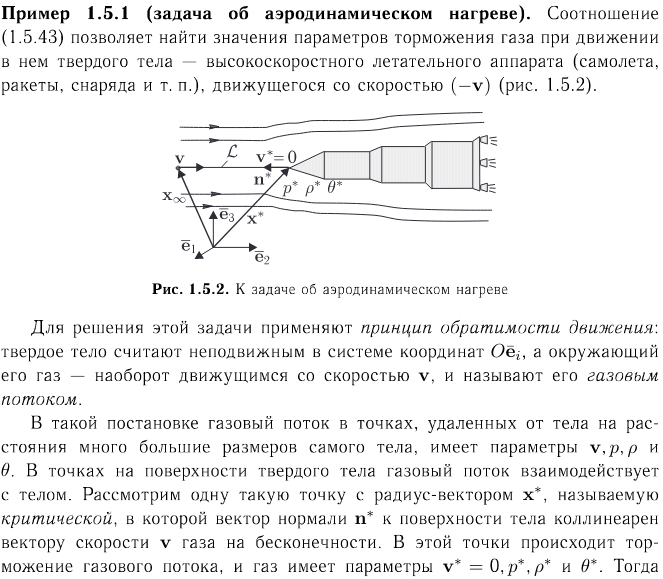
\includegraphics[width=0.7\linewidth]{img/50_01.png}
\end{figure}
\begin{figure}[H]
  \centering
  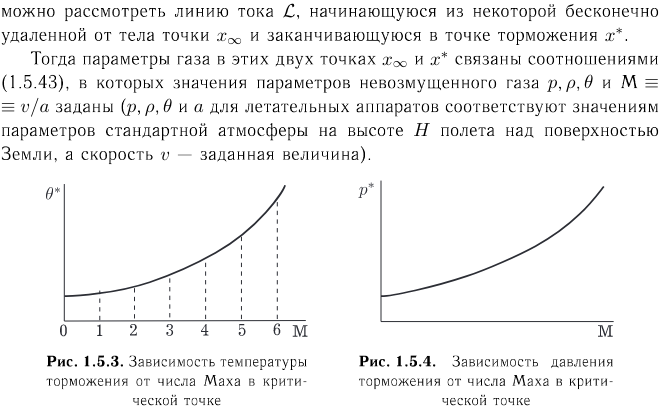
\includegraphics[width=0.7\linewidth]{img/50_02.png}
\end{figure}

Упомянутые соотношения (1.5.43):
\begin{align*}
  \dfrac{p}{p^*} &= \left( 1 + \dfrac{k-1}{2} M^2 \right)^{- k / (k-1)}, \\
  \dfrac{\rho}{\rho^*} &= \left( 1 + \dfrac{k-1}{2} M^2 \right)^{-1 / (k-1)}, \\
  \dfrac{\theta}{\theta^*} &= \left( 1 + \dfrac{k-1}{2} M^2 \right)^{-1}.
\end{align*}

\que{Трубка тока. Задача об установившихся одномерных течениях в соплах, простое сопло, сопло Лаваля.}


\end{document}
